\documentclass[a4paper,12pt, twoside]{NITKReport}
\usepackage[utf8]{inputenc}
\usepackage{underlin}
\usepackage{url}
\usepackage{comment}
\usepackage{cite}
\usepackage[authoryear,round,longnamesfirst]{natbib}
%\setcitestyle{notesep={; }, aysep={ }}
%\renewcommand*{\nameyeardelim}{\addspace}
\setcitestyle{aysep={}}
\usepackage{amsthm}   \theoremstyle{definition} \newtheorem{definition}{Definition}[section]
\usepackage{nomencl}
%\usepackage{pdfpages,caption}
\usepackage{longtable}
\usepackage{titlesec}
\usepackage{titletoc}
\usepackage{algorithmic}
\usepackage{amsthm}
\newtheorem{example}{Example}
%\usepackage[linesnumbered,ruled,vlined]{algorithm2e}
\titlecontents*{chapter}% <section-type>
[0pt]% <left>
{}% <above-code>
{\bfseries\chaptername\ \thecontentslabel \quad}% <numbered-entry-format>
{\bfseries\\\quad}% <numberless-entry-format>
{\bfseries\hfill\contentspage}
\usepackage[normalem]{ulem}
\usepackage{hyperref}
\usepackage{float}
\usepackage{caption}
\usepackage{parskip}
\setlength{\parindent}{20pt}
\usepackage{setspace}
\usepackage{graphicx}
\usepackage[linesnumbered,ruled]{algorithm2e}
\usepackage{color}
\usepackage{epsfig}
\usepackage[cmex10]{amsmath}
\usepackage{graphicx,wrapfig,lipsum}
%\usepackage{algorithmicx,algorithm}
\usepackage{graphicx}
\usepackage{color}
\usepackage{epsfig}
\usepackage{multirow}
%\usepackage{mathtools}
\usepackage{amsmath,amsthm}

\usepackage{amsfonts}
\usepackage{amssymb}
\usepackage{subfig}
\usepackage{nomencl}
\usepackage{graphicx,wrapfig,lipsum}
\usepackage{float}
\usepackage{lipsum}
\usepackage{booktabs}

\usepackage{booktabs,caption,fixltx2e}
\usepackage{threeparttable}  
\usepackage{booktabs}
\usepackage{multirow}
\usepackage{adjustbox}


% % % % % % % % % % % % % % % % % % % % % % % % % % % % % % % % % % % % % % %

\usepackage{array}
\newcolumntype{L}[1]{>{\raggedright\let\newline\\\arraybackslash\hspace{0pt}}m{#1}}
\newcolumntype{C}[1]{>{\centering\let\newline\\\arraybackslash\hspace{0pt}}m{#1}}
\newcolumntype{R}[1]{>{\raggedleft\let\newline\\\arraybackslash\hspace{0pt}}m{#1}}

\usepackage[linesnumbered,ruled]{algorithm2e}
\usepackage{marvosym}
\usepackage{mathtools}
%\bibliographystyle{unsrtnat}
%\usepackage[numbers,sort&compress]{natbib}
%\usepackage[numbers,super]{natbib}
\usepackage{hyperref}
\usepackage{blindtext}
\usepackage{graphicx}
%\graphicspath{ {images/} }
%package that were included on demand
\usepackage{authblk} % for affil
\usepackage{booktabs} % for table work
\usepackage{amsfonts} % for mathbb
\usepackage{enumitem} % for custom enumerate
\usepackage{float}

\usepackage{booktabs,caption,fixltx2e}
\usepackage{threeparttable}  
\usepackage{booktabs}
\usepackage{multirow}
\usepackage{adjustbox}

\usepackage{lipsum}% http://ctan.org/pkg/lipsum

\usepackage{bm}
\usepackage{tabularx}


\usepackage{url}
\usepackage{amsmath}
\providecommand{\keywords}[1]
{
  \small	
  \textbf{\textit{Keywords---}} #1
}
%%%%%%%%%%%%%%%%%%%%%%%%%%%%%%%%%%%%%%%%%%%%%%%%%%%%%%%%%%%%%%%%%%%%%%%%%%%%%%%%%%%%%%%%%%%%%%%
\usepackage{tikz}
\usepackage{pgfplots}

\pgfplotsset{compat=newest}
\usetikzlibrary{shapes.geometric,arrows,fit,matrix,positioning}
\tikzset
{
	treenode/.style = {circle, draw=black, align=center, minimum size=1cm},
	subtree/.style  = {isosceles triangle, draw=black, align=center, minimum height=0.5cm, minimum width=1cm, shape border rotate=90, anchor=north}
}


\usetikzlibrary{calc}
\newcommand\HRule{\rule{\textwidth}{1pt}}
%%%%%%%%%%%%%%%%%%%%%%%%%%%%%%%%%%%%%%%%%%%%%%%%%%%%%%%%%%%%%%%%%%%%%%%%%%%%%%%%%%%%%%%%%%%%%%%
%\usepackage{algorithm}

%\usepackage{algpseudocode}
\usepackage[linesnumbered,ruled]{algorithm2e}

\newtheorem{theorem}{Theorem}[section] \newtheorem{corollary}{Corollary}[theorem] \newtheorem{lemma}[theorem]{Lemma}

%\newtheorem{theorem}{Theorem}
%\newdefinition{definition}{Definition}
\newtheorem{prop}{Proposition}


\renewcommand{\bibname}{REFERENCES}
%\setcitestlye{aysep={}}
%\renewcommand*{\nameyeardelim}{\addspace}
\thispagestyle{empty}
\newpage
\tolerance=1
\emergencystretch=\maxdimen
\hyphenpenalty=10000
\hbadness=10000

\newpage

\let\oldemph\emph
\renewcommand\emph[1]{{\fontsize{13pt}{14pt}\selectfont\oldemph{#1}}}
\newcommand{\algorithmfootnote}[2][\footnotesize]{%
	\let\old@algocf@finish\@algocf@finish% Store algorithm finish macro
	\def\@algocf@finish{\old@algocf@finish% Update finish macro to insert "footnote"
		\leavevmode\rlap{\begin{minipage}{\linewidth}
				#1#2
			\end{minipage}}%
		}%
	}
	
	\DeclareMathAlphabet{\mathcal}{OMS}{cmsy}{m}{n}

\allowdisplaybreaks
\begin{document}
	
	\pagenumbering{gobble}
	
	\newcommand{\thesistitle}{Unsupervised Face Recognition Using One-Shot Learning}
	\newcommand\textlcsc[1]{\textsc{\MakeLowercase{#1}}}
	\newcommand{\regno}{16IS18F}
	\newcommand{\authorname}{RaviRaaja L}
	
	
	
	
	
	% --------------Title Page---------------------------%
	\begin{titlepage}
		\begin{center}
			{\textlcsc{\LARGE \thesistitle}}\\
			\vspace{20.5pt}
			
			%{\Large SAR IMAGES}\\
			%\vspace{40pt}
			
			Thesis\\
			\vspace{10pt}
			{\emph {Submitted in partial fulfillment of the requirements for the degree of}} \\
			\vspace{20pt}
			{\Large MASTER OF TECHNOLOGY}\\
			\vspace{10pt}
			in\\
			\vspace{10pt}
			{ \Large COMPUTER SCIENCE AND ENGINEERING - INFORMATION SECURITY}\\
			\vspace{25pt}
			\textit {by} \\
			\vspace{10pt}
			{\Large RaviRaaja L}\\ 
			{(Reg. No.: \regno)}\\
			\vspace{1CM}
			\includegraphics*[height=1.75in,width=1.75in]{NITK-Emblem.png}\\
			\vspace{1cm}
			\MakeUppercase{{\large Department of Computer Science \& Engineering}}\\
			\vspace{0.2cm}
			\MakeUppercase{{\large National Institute of Technology Karnataka, Surathkal}}\\
			\vspace{0.2cm}
			\MakeUppercase{{\large Mangalore - 575025}}\\
			\vspace{.2cm}
			\MakeUppercase{{\large JUNE 2018}}\\
		\end{center}
	\end{titlepage}
	% --------------Title Page---------------------------%
	
	%---------------Cover Page----------------------------%
	\begin{titlepage}
		\begin{center}
			\vspace{14.5pt}
			{\textlcsc{\LARGE \thesistitle}}\\
			\vspace{4.5pt}
			%{\Large SAR IMAGES}\\
			%\vspace{20pt}
			\vspace{20pt}
			\textit {by} \\
			\vspace{20pt}
			{\Large {RaviRaaja L}}\\ 
			{(Reg. No.: \regno)}\\
			\vspace{15pt}
			{\em Under the Guidance of} \\
			\vspace{10pt}
			Dr. Jeny Rajan\\
			Assistant Professor\\
			Department of CSE\\
			\vspace{1.5cm}
			\vspace{-0.25in}
			{THESIS}  \\
			\vspace{1.0cm}
			{\emph {Submitted in partial fulfillment of the requirements for the degree of}} \\
			\vspace{25pt}
			{\Large {MASTER OF TECHNOLOGY}}\\
			\vspace{5pt}
			in\\
			\vspace{5pt}
			{ \Large {COMPUTER SCIENCE AND ENGINEERING - INFORMATION SECURITY}}\\
			\vspace{1.5cm}
			{\Large Department of Computer Science and Engineering }\\
			\vspace{0.2cm}
			{\Large National Institute of Technology Karnataka, Surathkal}\\
			\vspace{0.2cm}
			{\Large Mangalore - 575025}\\
			\vspace{0.5cm}
			{\large JUNE 2018}\\
		\end{center}
	\end{titlepage}
	%---------------Cover Page----------------------------%
	
	%---------------Declaration Page ----------------------%
	\newpage
	\thispagestyle{empty}
	
\begin{tikzpicture}[remember picture, overlay]
	\draw[line width = 2pt] ($(current page.north west) + (0.75in,-0.75in)$) rectangle ($(current page.south east) + (-1in,1in)$);
	\end{tikzpicture}
	\section*{\centering DECLARATION}
	%\begin{center}
	%	\emph{by the M.Tech student}
	%\end{center}
	I hereby \emph{declare} that the Thesis entitled 
	{\bf \thesistitle} which is being submitted to {\bf National Institute of Technology Karnataka, Surathkal}, 
	in partial fulfilment for the requirements of the award of degree of {\bf Master of Technology} in {\bf Computer Science and Engineering - Information Security} in the department of {\bf Computer Science and Engineering}, 
	is a \emph{bonafide report of the work carried out by me}. The material contained  in this report has not been submitted at any other University or Institution for the award of any degree.
	
	\vspace{1.0in}
	\begin{flushright}
		\textbf{\regno, RaviRaaja L}\\ 
		\vspace{1.0cm}
		.........................................................\\
		(Register Number, Name and Signature of the student)\\
		%\vspace{1cm}
		Department of Computer Science and Engineering
	\end{flushright}
	
	\vspace{0.2in}
	\begin{flushleft}
		Place : NITK, Surathkal\\
		Date  :
	\end{flushleft}
	%---------------Declaration Page-----------------------%
	
	% --------------Certificate page----------------------%
	\newpage
	\thispagestyle{empty}
	\begin{tikzpicture}[remember picture, overlay]
	\draw[line width = 2pt] ($(current page.north west) + (1in,-1in)$) rectangle ($(current page.south east) + (-0.75in,1.25in)$);
	\end{tikzpicture}
	
	\section*{\centering CERTIFICATE}
	This is to \emph{certify} that the Thesis entitled 
	{\bf \thesistitle} 
	submitted by {\bf RaviRaaja L} (Register number: \regno) as the 
	record of the work carried out by him, is \emph{accepted as the  
		P.G Major Project Thesis submission} in partial fulfilment for 
	the requirements of the award of degree of {\bf Master of Technology} 
	in {\bf Computer Science and Engineering - Information Security} in the department of {\bf Computer Science and Engineering} 
	at {\bf National Institute of Technology Karnataka, Surathkal} during the 
	academic year 2017-2018.
	
	
	\vspace{1.4in}
	\begin{tabular}{ll}
		\hspace{-1cm}{...............................}&\hspace{6cm}{...............................}\\
		\hspace{-1cm}\bf{Dr.Jeny Rajan}  & \hspace{6cm}\textbf{Alwyn R. Pais}			\\
		\hspace{-1cm}\bf{Project Guide}     &\hspace{6cm}\bf{Chairman-DPGC}\\
		\hspace{-1cm}\bf{Department of CSE,}	  &\hspace{6cm}\bf{Department of CSE,}			\\
		\hspace{-1cm}\bf{NITK Surathkal}	  &\hspace{6cm}\bf{NITK Surathkal}\\
		
	\end{tabular}
	
	
	% --------------Certificate page----------------------%
	
	
	%------------------Ack page ---------------------------%
	\newpage
	%\pagenumbering{roman}
	\pagestyle{plain}
	\thispagestyle{empty}
	\section*{\centering ACKNOWLEDGEMENT}
	
	I take this opportunity to express my deepest gratitude and appreciation to all those who have helped me directly or indirectly towards the successful completion of this project.\\ \\
	I would like to express my gratitude to my guide Dr.Jeny Rajan, Department of Computer Science and Engineering, National Institute of Technology Karnataka, Surathkal for his continuous encouragement and support in carrying out my project work. He has continuously mentored my work and corrected my mistakes, without which it would have been difficult to carry out this project. I would like to thank him for all the help and necessary suggestions that he has always provided me with.\\ \\
	I express my deep gratitude to project coordinator Mr.Mahendra Pratap Singh, Department of Computer Science and Engineering, National Institute of Technology Karnataka, Surathkal for his constant co-operation, support and for providing necessary facilities throughout the M.Tech. program.\\ \\
	I would also like to thank all the supporting staff members of the department of Computer Science and Engineering. Without their timely help and support, it would not have been possible to carry out my project.
	
	\vspace{1cm}
	\begin{tabular}{ll}
		\hspace{-1cm}{\textbf{Place:} Surathkal} &\hspace{7cm}{RaviRaaja L}\\
		\hspace{-1cm}{\textbf{Date:} June 2018}	&\hspace{7cm}\bf{}		\\
		
	\end{tabular}
	
	
	%------------------Ack page ---------------------------%
	
	\newpage

\begin{abstract}

The ability to recognize and remember individuals is crucial task and has important implications for the evolution of human social behavior, particularly complex interactions between groups. Recently, the role of mass media in shaping public perceptions at scale has come under increasing scrutiny. Implementation of face recognition at large scale involves in face detection and feature extraction using deep convolutional neural network models for clustering the features. We evaluated the effectiveness of deep convolutional neural network architectures and clustering approaches both qualitative and quantitative metrics. However, the conventional softmax loss of Deep CNNs for the most part does not have potential of segregation. To address this issue modified loss functions are used recent years, for example, large margin softmax loss, large margin cosine loss, center loss. All these improved losses shared same idea; maximizing inter-class variance and minimizing intra class variance. In this project we propose a method to deploy unsupervised face recognition using combination of above improved loss functions and customized Deep CNN training methodology.
\newline
\newline
\keywords{\textit{Face Recognition, Face Detection, Deep Convolutional Neural Networks, Center Loss, Large Margin Softmax Loss, Large Margin Cosine Loss, Softmax Loss.}}

\end{abstract}


\begin{spacing}{1.2}
\tableofcontents
\end{spacing}
\newpage

\renewcommand{\listfigurename}{LIST OF FIGURES}
\renewcommand{\listtablename}{LIST OF TABLES}
\pagenumbering{roman}
\addcontentsline{toc}{section}{List of Figures}

\listoffigures
\newpage
%\addcontentsline{toc}{chapter}{\listfigurename}
%\listoffigures   \listtablename

\addcontentsline{toc}{section}{List of Tables}
%\pagenumbering{roman}
\listoftables
\newpage
%\newpage
%\addcontentsline{toc}{chapter}{\small List of Abbreviations}
%\addcontentsline{toc}{section}{Abbreviations}
%\textbf{\LARGE List of Abbreviations}\\
%\makenomenclature
%
%\nomenclature{SNA}{Social Network Analysis}
%GnN Girvan and Newman\\
%RnB Riechardt and Bronholdt
%Rnv Ronhovode and Nussinov\\
%Spec Spectral Clustering\\

%\cleardoublepage
%\pagestyle{fancy}
% with this we ensure that the chapter and section
% headings are in lowercase.

\begin{comment}
\renewcommand{\chaptermark}[1]{%
	\markboth{#1}{}}
\renewcommand{\sectionmark}[1]{%
	\markright{\thesection\ #1}}
\fancyhf{} % delete current header and footer
\fancyhead[LE,RO]{\bfseries\thepage}
\fancyhead[LO]{\bfseries\rightmark}
\fancyhead[RE]{\bfseries\leftmark}
\renewcommand{\headrulewidth}{0.5pt}
\renewcommand{\footrulewidth}{0pt}
\addtolength{\headheight}{0.5pt} % space for the rule
\fancypagestyle{plain}{%
	\fancyhead{} % get rid of headers on plain pages
	\renewcommand{\headrulewidth}{0pt} % and the line
}
\end{comment}
\renewcommand{\chaptername}{CHAPTER}
\pagenumbering{arabic}

\chapter{Introduction}
\label{chap1}

Face Recognition is crucial task and has important implications for the evolution of human social behavior, particularly complex interactions between groups. Recently, the role of mass media in shaping public perceptions at scale has come under increasing scrutiny. Notably, many of the questions researchers wish to ask about mass media revolve around the questions of who, or making conclusions based on the identifying unique individuals on screen. The goal of this project is to automatically cluster and recognize unique faces for face verification and recognition where dataset is composed of images from various digital medium with different noise levels, image intensity and contrast. Main objective of this project is to come up with a novel deep convolutional neural network architecture which does on-line training on real time images and also to implement a working model as agile software to perform face verification and face clustering using online training.  
	
\section{Problem Statement}
\label{prob}
	 In the world of face recognition, however, large scale public datasets have been lacking largely due to this factor such as advances in the community remain restricted to Internet giants such as Facebook and Google etc. Facebook [\cite{1}] and Google [\cite{2}] have implemented supervised face recognition as proprietary tools using massive analytics and private datasets trained on Deep CNNs, tech giants uses existing data on generative models to improve the dataset variance adaptively. In reality, greedy approaches are emphasized on training Deep CNN models. Using very less dataset for each instances of face images and to obtain good recognition accuracy, which is also called as one shot learning problem. In order to do one shot learning with better discriminative impacts, it is necessary to use an objective function which has tendency to discriminate the features to larger extent such that inter class variance is maximized. The problem with available standard dataset includes negligible number of instances of faces to train deep networks. Annotated images with high class imbalance and varying noise levels makes face verification less accurate. Though datasets scarcity problem can be solved by manually adding face images by scrapping the google search results, appended by using Haar cascade approaches [\cite{viola2001rapid}], face detection has the problem of translational variance such as face angle exposure. Major issues in this project can be listed as follows designing optimal real time clustering algorithm for grouping similar faces and fine tuning approaches to deploy model as real-time application.

		
	\section{Motivation}
	\label{moti}
	Face images are primary source to understand human behavior can impact the economy of the country. For example, [\cite{3}] china has implemented nationwide face recognition system that detects the faces and categorize them according to rules of centralized surveillance system, along side by understanding where people travel, eat, understanding their daily routine patterns helps the government to design better business and industrial policies to improve economy of country. 
In September 2012, the Internet Archive launched the TV News Archive, a repository of 500,000+ TV news broadcasts aired since 2009 (2017). Closed captions are also provided alongside the video, allowing for richer interactions with the video data. Researchers hope to enable users to ask identity-based queries about this data, such as who appeared on Fox News and discussed immigration the greatest number of times in January. The FBI’s Next Generation Identification System uses facial recognition to compare images from crime scenes with a national database of mugshots. Police forces across the United States have been using traditional algorithm-based techniques for several years to predict where crimes are likely to occur. By making face recognition technology which is completely unsupervised and availing it for people as RESTful services will be useful to deploy secure home surveillance system and also useful for government to understand the patterns of people behaviors. The problem is divided into three objectives which are face detection, feature extraction ,face clustering and face verification.

	
\section{Contributions}
\label{contri}
 The major contribution are as follows:
  
\begin{itemize}
\item Deploying deep learning models as agile software is a challenging task. In this project, unsupervised face recognition system using deep convolutional neural networks is deployed with validation accuracy of 98\% on real time face images using tensorflow as back end pipeline for production. Implementation of combined discriminative learning objective functions like center loss with softmax [\cite{wen2016discriminative}], triplet loss [\cite{schroff2015facenet}], Quadruplet loss [\cite{chen2017beyond}] and margin cosine loss[\cite{DBLP:journals/corr/abs-1801-09414}] have been implemented to train the model and to produce better discriminative results.
\item Implementation of wrapper module using python on MTCNN a novel face detection approach is performed in this project to capture the faces from real time images and align them irrespective of facial orientation and noise levels, given weights for pre-trained MTCNN model. [\cite{xiang2017joint}]
\item Analysis of kmeans++ clustering, DBScan clustering, Guassian clustering models and Rank order clustering with silhoutte scores as inertia.
\item Implementation of light weight graph based custom clustering technique has been deployed to solve problem of unsupervised face recognition in large scale. 
\item Automatic intuitive training of deep convolutional neural network without over fitting the model. [\cite{DBLP:journals/corr/CogswellAGZB15}]
\item Implementation of data visualization technique t-SNE (Stochastic Neighborhood embedding) to visualize whether embeddings are suitable for clustering and retraining model. [\cite{maaten2008visualizing}] 

\end{itemize}
	
\section{Organization of the thesis}
	Chapter~\ref{chap1} gives a brief introduction along with formal problem statement in section~\ref{prob} and motivation in section~\ref{moti} and the contributions of this work in section~\ref{contri}. Chapter~\ref{chap2} tabulates the literature on research over unsupervised face recognition. Chapter~\ref{chap3} includes the proposed solution ,various deep CNN architecture experimented and Clustering approaches used. Chapter~\ref{chap4} Includes strategy on deployment of Deep CNN for unsupervised face recognition. Chapter~\ref{chap5} includes conclusion and further research ideas to extend the research.  
	
\newpage
\chapter{Liturature Survey}
\label{chap2}

\section{Face Clustering}
\begin{table}
  \centering
\begin{tabular}{ |p{3cm}|p{3cm}|p{2.5cm}|p{2cm}|p{2cm}|}
 \hline
 Publication & Features & Clustering Methods & \#Face images & \#Subjects\\
 \hline
 [\cite{ho2003clustering}] & Gradient and Pixel Intensity Features& Spectral Clustering & 1386 & 66\\
 \hline
 [\cite{zhao2006automatic}] & 2DHMM $+$ contextual & Hierarchical Clustering & 1500 & 8\\
  \hline
 [\cite{cui2007easyalbum}] & LBP, clothing color $+$ texture & Spectral Clustering & 400 & 5\\
  \hline
 [\cite{tian2007face}] & Image $+$ Contextual & Partial Clustering & 1147 & 34\\
  \hline
[\cite{zhu2011rank}] & Learning based descriptor & Rank order Clustering & 1322 & 53\\
  \hline
  Vidal and Favaro [\cite{li2015structured}] [\cite{zhang2014jointly}] & Joint subspace learning & Similarity based clustering & 2432 & 38\\
 \hline
\end{tabular}
\caption{Papers on Face clustering}\label{table:papers}
\end{table}

\par The below table ~\ref{table:papers} lists prior work on face clustering with the face representation and clustering algorithm used as well as the largest dataset size used in terms of face images and the number of subjects. [\cite{ho2003clustering}] developed variations on spectral clustering by computing the probability that two face images are of the same object. [\cite{zhao2006automatic}] clustered personal photograph collections by combining a variety of contextual information including time based clustering, and the probability of faces of certain people to appear together in images. They also used identity estimates from a  Hidden  Markov  model,  and  hierarchical  clustering results based on body detection.[\cite{cui2007easyalbum}] developed a semi-automatic tool for annotating photographs,  which employs clustering as an initial method for organizing photographs. They extracted features from detected faces and color and texture features were extracted, and then spectral
clustering was performed and evaluated on a dataset consisting of 400 photographs of 5 subjects. [\cite{tian2007face}] refined this approach by incorporating a
probabilistic clustering model which used a junk class that allowed the algorithm to discard clusters that do not have tightly distributed samples. [\cite{zhu2011rank}] developed a dissimilarity measure based on two faces being in each others nearest neighbor lists, and perform hierarchical clustering based on the resulting rank-order distance.  However, this clustering method was evaluated on small datasets (approximately 1,300 face images).To the best of our knowledge,this study is the first to attempt to do unsupervised identity  clustering on a large scale (infinite images). From the literature review, it is  clear that most studies used pre-extracted faces from standard database rather than using real time data in my case, model is trained online using clustering output on real time data which follow various noise levels. Moreover, the 128-byte feature extractors we use are significantly smaller than the features employed  in  other  studies  allowing  for  higher  efficiency and scalability.

\section{Supervised Face Detection and Recognition}
\par Semi supervised learning approaches is used to solve problem at first stage by obtaining embeddings from Deep CNN, so it is necessary to analyze the supervised approaches which uses deep convolutional neural networks which works well for face classification. Thus the experiments can be performed from selected optimal model. Below table.~\ref{table:papers1} list the prior work on face image classification. In 2015, Google released technique to train models for classification problems on discriminating features,called FaceNet. FaceNet follows Inception V3[\cite{DBLP:journals/corr/SzegedyVISW15}] deep neural network architecture and have trained using the technique called as siamese network [\cite{Koch2015SiameseNN}], where two networks are used for training images which are identical and also share same weights. Objective function used is triplet loss where triplets of input images are used for training. Usage of this objective function results in extending distance or similarity between the two faces, such that if given two faces are different distance is increased and else reduced~\ref{triplet}. Inception architecture is highly preferred to obtain embeddings for clustering because using multiple features from multiple filters improve the performance of the network. Other than that, there is another fact that computational complexity on making convolution operations is less costly, makes the inception architecture better than others. All the architectures prior to inception, performed convolution on the spatial and channel wise domain together. By performing the 1x1 convolution, the inception block is doing cross-channel correlations, ignoring the spatial dimensions. This is followed by cross-spatial and cross-channel correlations via the 3x3 and 5x5 filters. Thus inception based models are decided to be used to solve the problem of unsupervised face recognition. Same year Oxford visual Geometry Group performed experiments on conventional CNN model with triplet loss this results in better classification accuracy than facenet. In 2016 CMU have implemented preprocessing techniques to feed into same inception variants like architecture [\cite{amos2016openface}] and trained in distributed way to make the weights used for deploying face recognition in mobile applications in supervised way. Thus Google and Oxford has access to extensive amount of private face dataset, training and validation accuracy of the model was more compared to Open face [\cite{amos2016openface}].[\cite{chen2017beyond}] introduced objective function that made use of four images such as anchor, positive, negative and more-negative to train the DCNN architecture similar to triplet loss but this process have very high time complexity compared to training a model with triplet loss. Behalf of face recognition and face clustering, major problem also lays in face detection because conventional face detection approaches performs well only on standard database. For real time data set [\cite{zhang2016joint}] introduced new deep convolutional neural network approach named as multi task CNN which is considered as state of art face detection algorithm, thus in this project some more preprocessing techniques are added like usage of laplacian filter to remove blur.  

\begin{table}
  \centering
\begin{tabular}{ |p{3cm}|p{3cm}|p{2.5cm}|p{2cm}|p{2cm}|}
 \hline
 Publication & Feature Extraction Methods & Objective function & AUC\\
 \hline
 Google Brain [\cite{schroff2015facenet}] & Siamese Network and Inception V3 & Triplet Loss & 0.98\\
 \hline
 Deep Face [\cite{parkhi2015deep}] & Alex Net without Local Response Normalization and other variations [\cite{DBLP:journals/corr/SimonyanZ14a}] & Triplet loss & 0.99 \\
\hline
  [\cite{amos2016openface}] & Affine Transformation and DCNN & Triplet Loss & 0.973\\ 
 \hline
 [\cite{chen2017beyond}] & Margin-based hard negative mining & Quadruplet Loss & 0.98 \\
 \hline
 [\cite{zadeh2017convolutional}] & Preprocessing and Correlation Network & Land mark detection approach & NIL \\ 
 \hline
[\cite{zhang2016joint}] & Multi Task cascade convolutional Neural Network & Face Detection and orientation  & NIL \\
\hline
\end{tabular}
\caption{Papers on Supervised Face Classification and Land mark detection}\label{table:papers1}
\end{table}




\newpage
\chapter{Proposed Solution}
\label{chap3}
\label{solution}
\section{Overview}
\par Semi supervised learning is the technique opted as first step to solve the problem of unsupervised face recognition. Semi supervised learning with respect to face recognition includes steps such as training standard face images with annotations. As mentioned earlier traditional softmax loss function will not make much impact in discriminating th facial features, usage of appropriate objective function and on training real-time cropped face images using deep convolutional neural network, which is also called as supervised learning. Dataset is trained until optimized validation accuracy is obtained. Cropped face images irrespective of its image features when passed into trained deep CNN to obtain embeddings and clustering those embeddings outputted from the Deep CNNs resulted as labels, with which respect to labels medoid is computed to represent the entire unique cluster. Face verification is performed by a forward pass of cropped face which has to be verified into Deep CNN to obtain embeddings and compare the confidence with all medoids (minimal thresholded confidence value obtained previously). Thus to improve the embeddings patterns to follow principle of high inter class variance and low intra class variance, deep CNN is re-trained in a supervised mode with obtained labels to get model tuned and to produce densely packed embeddings.

\par The widely used softmax loss in the training process often bring large intra-class variations, and feature normalization is only exploited in the testing process to compute the pair similarities.  To bridge the gap, we impose the modified intra-class cosine similarity between the features and weight vectors, which is deployed with combination of softmax loss larger than a margin in the training step, and extend it from four aspects. First, we explored the effect of a hard sample mining strategy. To alleviate the human labor of adjusting the margin hyper-parameter, a self-adaptive margin updating strategy is proposed. Then, a normalized version is given to take full advantage of the cosine similarity constraint. Furthermore, we enhance the former constraint to force the intra-class cosine similarity larger than the mean inter-class cosine similarity with a margin in the exponential feature projection space. Cosine similarity and usage of center loss resulted in almost same accuracy and by comparing memory constrains center loss with softmax loss is used to trained the final model.

\subsection{Reason for using Deep CNN}
\par Recent year Deep CNNs are giving best results for the problem of image classification. Thus image-net challenge is considered as standard for ranking deep neural network model with respect to Top 5 classification accuracy. [\cite{NIPS2012_4824}] Deep convolutional neural networks are used for face recognition because faces image have high intraclass correlation. Intraclass correlation coefficient (ICC) [\cite{koch1982intraclass}] is an inferential statistic that can be used when quantitative measurements are made on units that are organized into groups. It describes how strongly units in the same group resemble each other. While it is viewed as a type of correlation, unlike most other correlation measures it operates on data structured as groups, rather than data structured as paired observations. In other words the Intraclass Correlation (ICC) assesses rating reliability by comparing the variability of different ratings of the same subject to the total variation across all ratings and all subjects.
\par There are many standard DCNN architecture available to perform classification problem on images, thus with respect to results of image-net challenge 2017,Squeeze and Excitation blocks are suggested to be used at deep layers of the network. Thus experiments are performed on different neural network architectures like ResNet50 [\cite{he2016deep}], VGG16 [\cite{DBLP:journals/corr/SimonyanZ14a}],Inception V3 [\cite{DBLP:journals/corr/SzegedyVISW15}], Xception [\cite{DBLP:journals/corr/Chollet16a}] etc., because of data scarcity and available dataset has different noise distribution ,intensity and contrast variation. The best results are obtained from usage if inception-Resnet v2 [\cite{DBLP:journals/corr/SzegedyIV16}].

%%%%%%%%%%
\section{Deep CNN Architecture}
\subsection{Pure Inception Blocks}
Older Inception models used to be trained in a partitioned manner, where each replica was partitioned into a multiple sub-networks in order to be able to fit the whole model in memory.  However, the Inception architecture is highly  tunable,  meaning  that  there  are  a  lot  of  possible changes to the number of filters in the various layers that do  not  affect  the  quality  of  the  fully  trained  network. In order to optimize the training speed,  we used to tune the layer sizes carefully in order to balance the computation between the various model sub-networks. In contrast, with the introduction of Tensor-Flow ,current models can be trained without partitioning the replicas. This is enabled in part by recent optimizations of memory used by back-propagation, achieved by carefully considering what tensors are needed for gradient computation and structuring the computation to reduce the number of such tensors. We have been relatively conservative about changing the architectural choices and restricted our experiments to varying isolated network components while keeping the rest of the network stable.  Not simplifying earlier choices resulted in networks that looked more complicated that they needed to be. In our newer experiments, for Inception-v4 it is decided to shed this unnecessary baggage and made uniform choices for the Inception blocks for each grid size.  Please refer to Fig.~\ref{9} for the large scale structure of the Inception-v4 network and refer Fig.~\ref{3},~\ref{4},~\ref{5},~\ref{6},~\ref{7} and ~\ref{8} for the detailed structure  of  its  components. All the convolutions not  marked with “V” in the figures are same-padded meaning that their output grid matches the size of their input. Convolutions marked with “V” are valid padded, meaning that input patch of each unit is fully contained in the previous layer and the grid  size  of  the  output  activation  map  is  reduced  accordingly.[\cite{DBLP:journals/corr/SzegedyIV16}]

\begin{figure}[h]
  \centering
    
    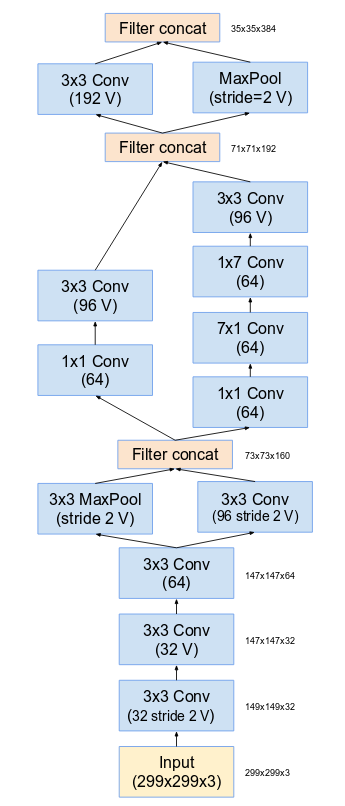
\includegraphics[height=21cm, width=8cm]{figure3.png}
    \caption{The blueprint for stem of the basic Inception-v4 and 
Inception ResNet-v2 systems. This is the input part of neural network [~\cite{szegedy2017inception}]. Cf. Figures ~\ref{9} and ~\ref{15}}
    \label{3}
  
\end{figure}

\begin{figure}[h]
\centering

    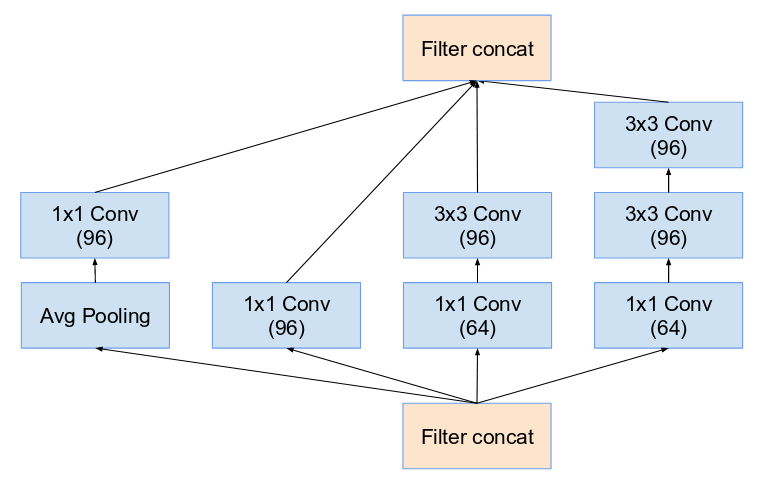
\includegraphics[height=8cm,width=15cm]{figure4.png}
    \caption{The  schema  for 35 x 35 grid  modules of the pure Inception-v4 network. This is the Inception-A block of Figure ~\ref{9}.~[\cite{szegedy2017inception}]}
    \label{4}
  
\end{figure}



\begin{figure}[h]
  \centering
  
    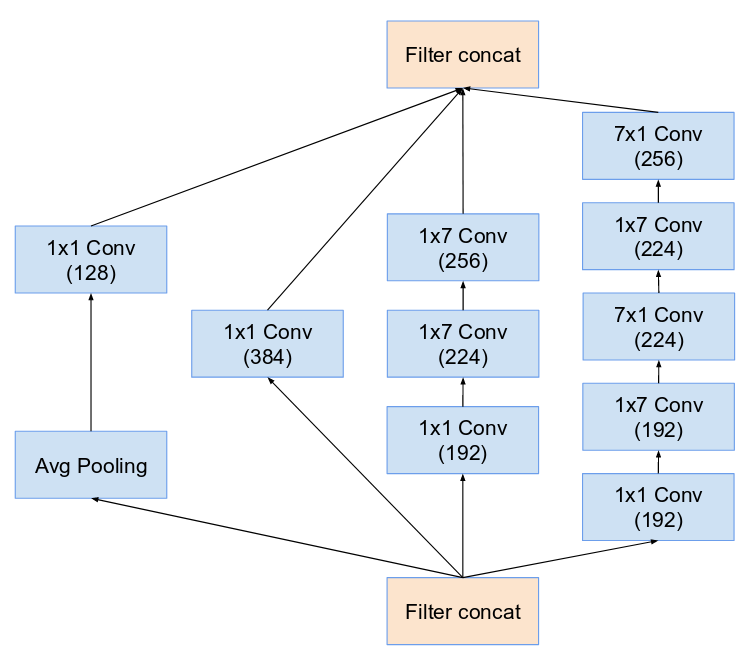
\includegraphics[height=10cm,width=15cm]{figure5.png}
    \caption{The  schema  for 17x17 grid  modules  of  the  pure Inception-v4 network. This is the Inception-B block of Figure ~\ref{9}.~[\cite{szegedy2017inception}]}
    \label{5}
 
 \end{figure}
 
 \begin{figure}
 \centering
 
    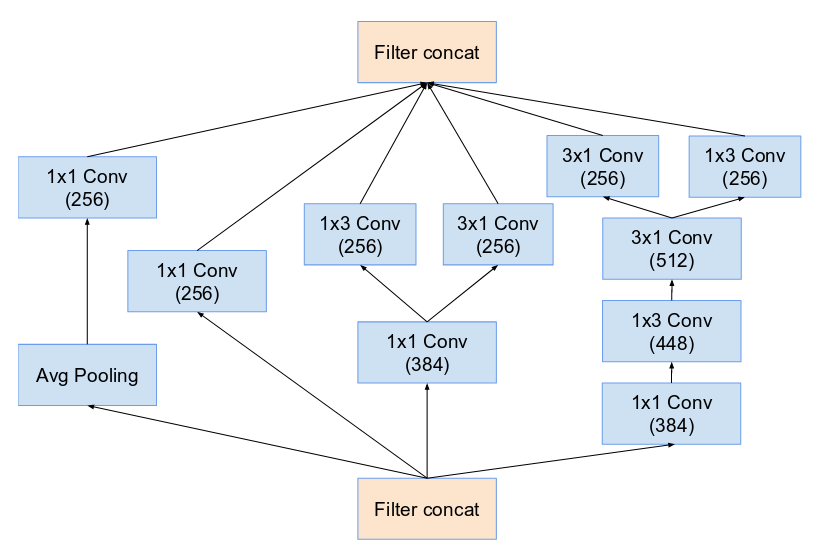
\includegraphics[height=10cm,width=16cm]{figure6.png}
    \caption{The schema for 8x8 grid modules of the pure Inception-v4 network. This is the Inception-C block of Figure ~\ref{9}.[~\cite{szegedy2017inception}]}
    \label{6}
  
\end{figure}

\begin{figure}[h]
  \centering
  
    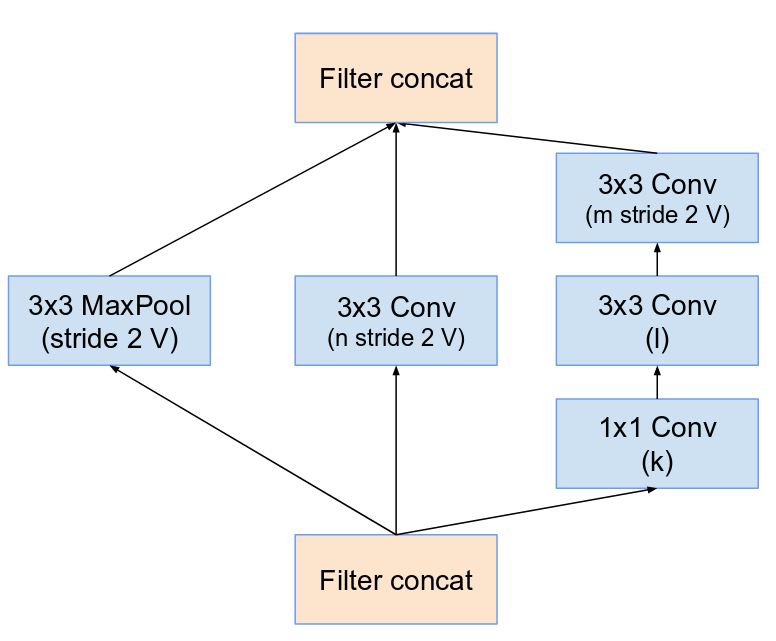
\includegraphics[height=8cm,width=15cm]{figure7.png}
    \caption{The schema for 35x35 to 17x17 reduction module. Different variants of this blocks (with various number of filters) are used in Figure ~\ref{9}, and ~\ref{15} in each of the new Inception(-v4, -ResNet-v1, -ResNet-v2) variants presented in this thesis. The k,l,m,n numbers represent filter bank sizes which can be looked up in Table ~\ref{table:number_of_filters}.[~\cite{szegedy2017inception}]}
    \label{7}
  
 \end{figure}
 
\begin{figure}
\centering
\begin{minipage}[b]{0.4\textwidth}
    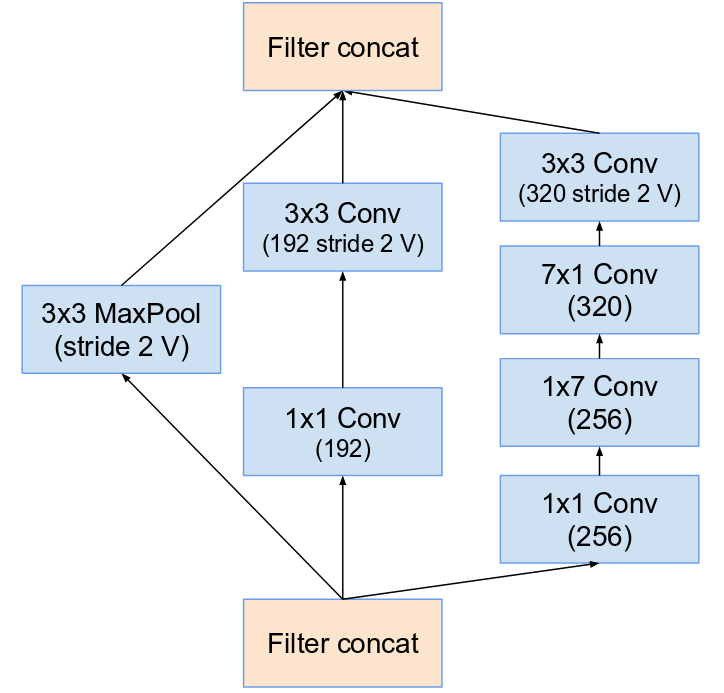
\includegraphics[height=9cm,width=8cm]{figure8.png}
    \caption{The schema for 17x17 to 8x8 grid-reduction module. This is the reduction module used by the pure Inception-v4 network in Figure ~\ref{9}.~[\cite{szegedy2017inception}]}
    \label{8}
  \end{minipage}
  \hfill
  \begin{minipage}[b]{0.4\textwidth}
 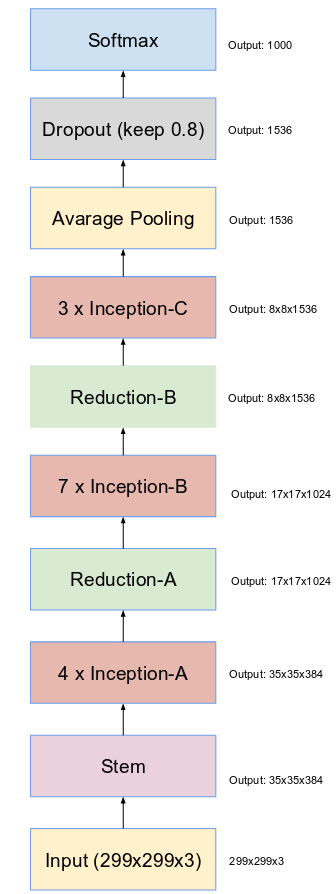
\includegraphics[height=19cm,width=8cm]{figure9.png}
    \caption{The overall schema of the Inception-v4 network. For the
detailed modules, please refer to Figures ~\ref{3}, ~\ref{4}, ~\ref{5}, ~\ref{6}, ~\ref{7} and ~\ref{8} for the detailed structure of the various components.[~\cite{szegedy2017inception}]}
    \label{9}
  \end{minipage}
\end{figure}


\begin{figure}[h]
  \centering
    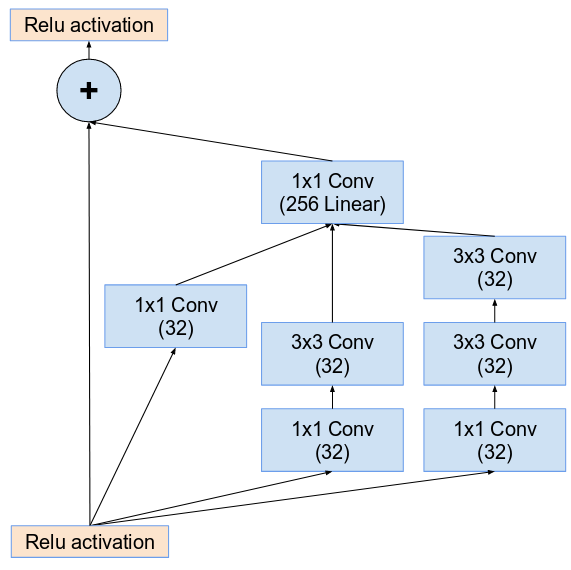
\includegraphics[height=10cm,width=13cm]{figure10.png}
\caption{The  schema  for 35x35 grid  (Inception-ResNet-A) module of Inception-ResNet-v1 network,[~\cite{szegedy2017inception}]}
\label{10}
\end{figure}

\begin{figure}[h]
  \centering
    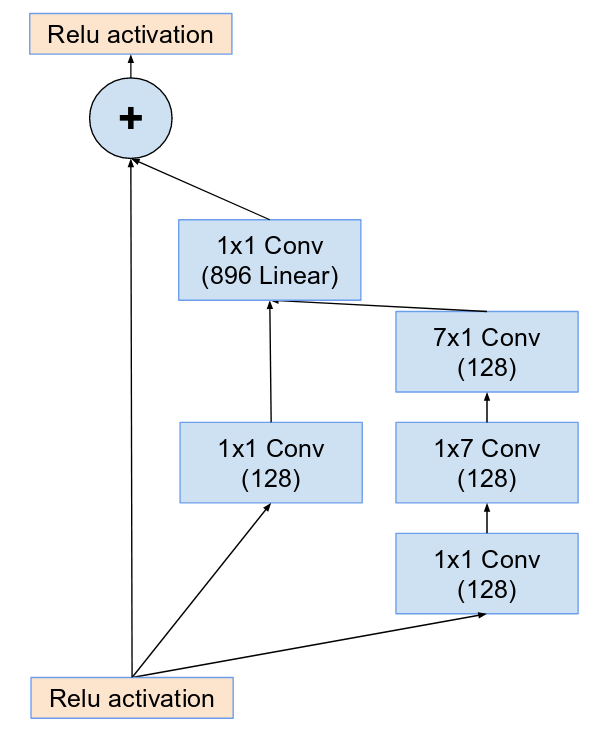
\includegraphics[height=10cm,width=13cm]{figure11.png}
    \caption{The  schema  for 17x17 grid  (Inception-ResNet-B) module of Inception-ResNet-v1 network.[~\cite{szegedy2017inception}]}
    \label{11}
 
\end{figure}


\begin{figure}

\centering
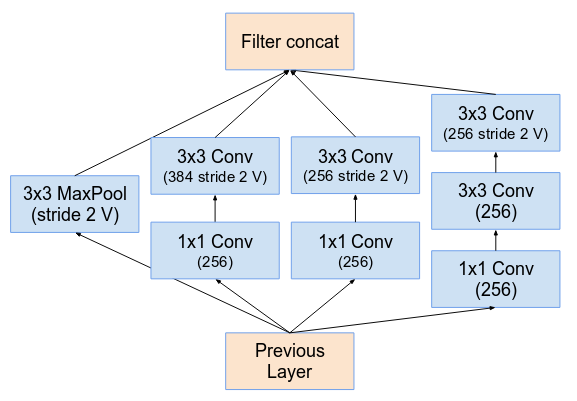
\includegraphics[height=10cm,width=13cm]{figure12.png}
    \caption{“Reduction-B” 17x17 to 8x8 grid-reduction module.This module used by the smaller Inception-ResNet-v1 network in Figure ~\ref{15}.~[\cite{szegedy2017inception}]}
\label{12}
\end{figure}

\begin{figure}[h]
  \centering
    
    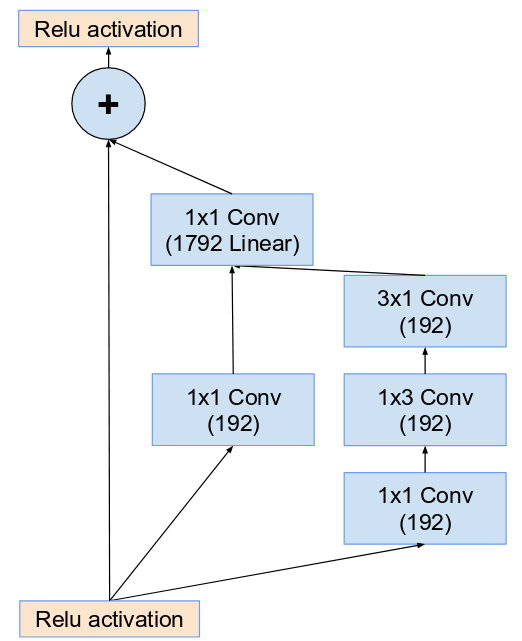
\includegraphics[height=10cm,width=13cm]{figure13.png}
    \caption{ The schema for 8x8 grid (Inception-ResNet-C) module of Inception-ResNet-v1 network.[~\cite{szegedy2017inception}]}
    \label{13}
   \end{figure}
 
\begin{figure}
\centering
\begin{minipage}[b]{0.4\textwidth}
   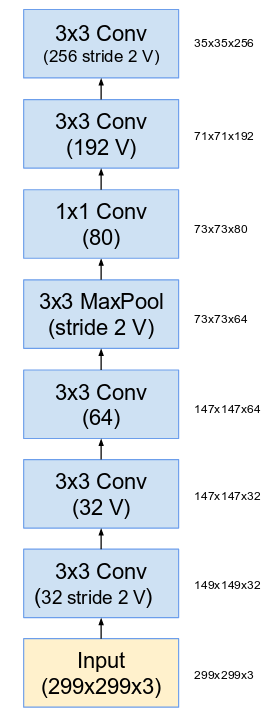
\includegraphics[height=15cm,width=6cm]{figure14.png}
    \caption{The stem of the Inception-ResNet-v1 network.[~\cite{szegedy2017inception}]}
    \label{14}
  \end{minipage}
  \hfill
  \begin{minipage}[b]{0.4\textwidth}
    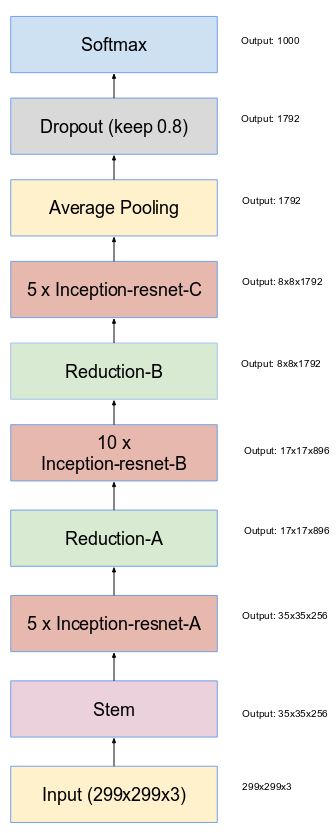
\includegraphics[width=\textwidth]{figure15.png}
    \caption{Schema   for   Inception-ResNet-v1   and   Inception-ResNet-v2 networks.  This schema applies to both networks but the underlying components differ.  Inception-ResNet-v1 uses the blocks as described in Figures ~\ref{14}, ~\ref{10}, ~\ref{7}, ~\ref{11}, ~\ref{12} and ~\ref{13}. Inception-ResNet-v2 uses the blocks as described in Figures ~\ref{3}, ~\ref{16},~\ref{7}, ~\ref{17}, ~\ref{18} and  ~\ref{19}. The output sizes in the diagram refer to the  activation vector tensor shapes of Inception-ResNet-v1.[~\cite{szegedy2017inception}]}
    \label{15}
  \end{minipage}
\end{figure}

\begin{figure}[h]
  \centering
    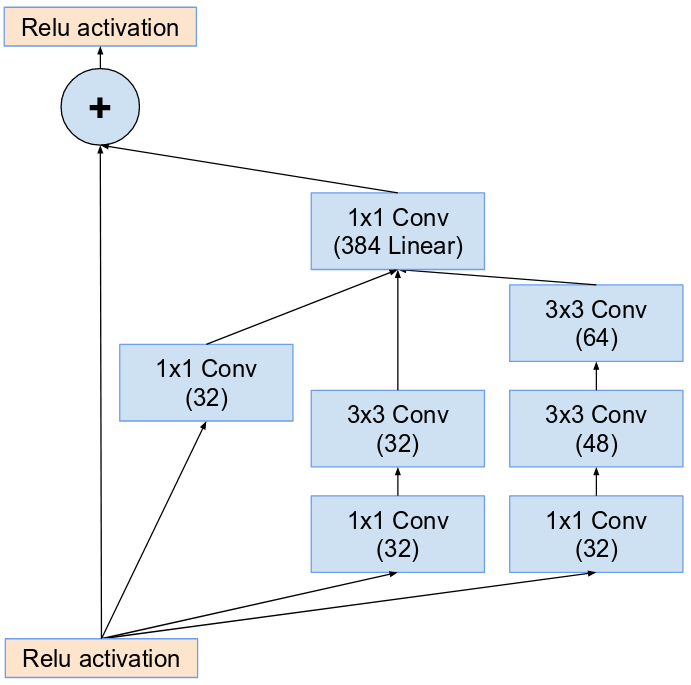
\includegraphics[height=10cm,width=13cm]{figure16.png}
    \caption{The  schema  for 35x35 grid  (Inception-ResNet-A) module of the Inception-ResNet-v2 network.[~\cite{szegedy2017inception}]}
    \label{16}

\end{figure}

\begin{figure}[h]
  \centering
   
    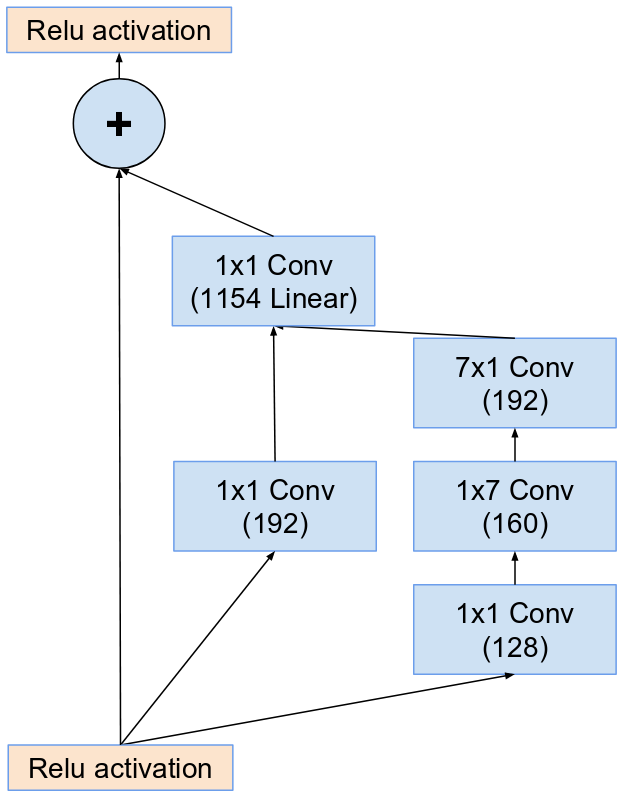
\includegraphics[height=10cm,width=13cm]{figure17.png}
    \caption{ The  schema  for 17x17 grid  (Inception-ResNet-B) module of the Inception-ResNet-v2 network.[~\cite{szegedy2017inception}]}
    \label{17}
 
 \end{figure}
 
 \begin{figure}[h]
\centering
    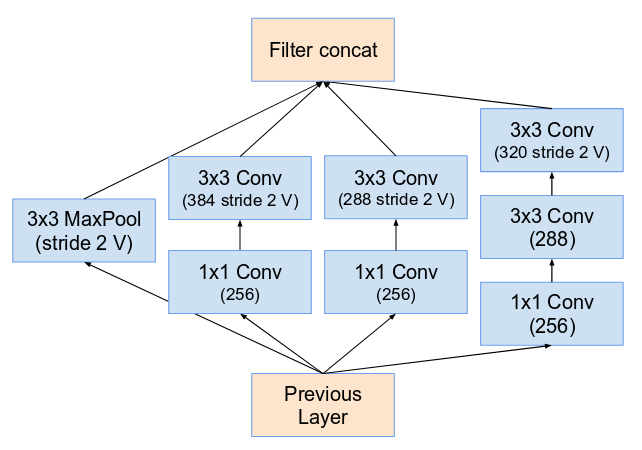
\includegraphics[height=10cm,width=13cm]{figure18.png}
    \caption{ The schema for 17x17 to 8x8 grid-reduction module. Reduction-B module used by the wider Inception-ResNet-v1 network in Figure ~\ref{15}.~[\cite{szegedy2017inception}]}
    \label{18}
 
\end{figure}

\begin{figure}[h]
  \centering
    
    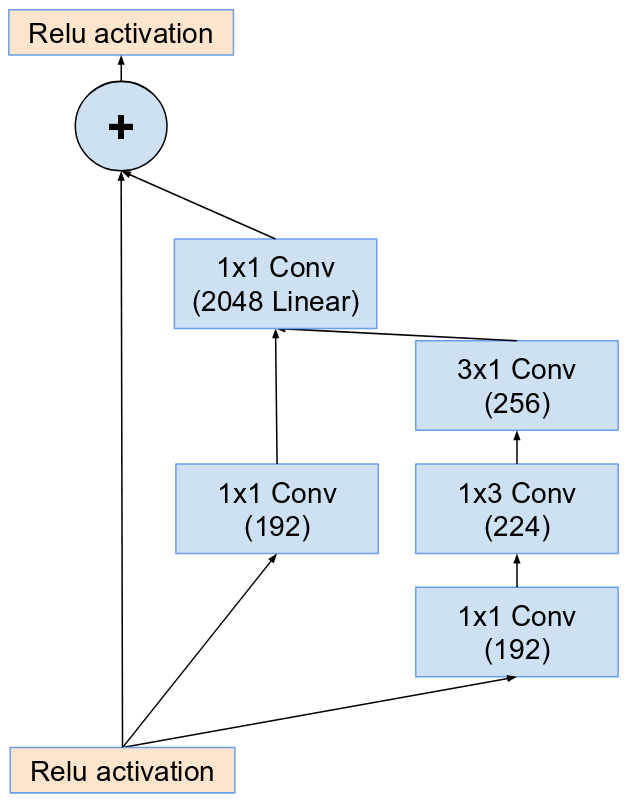
\includegraphics[height=10cm,width=13cm]{figure19.png}
    \caption{The schema for 8x8 grid (Inception-ResNet-C) module of the Inception-ResNet-v2 network.[~\cite{szegedy2017inception}]}
    \label{19}
  
  \end{figure}
\begin{figure}
\centering
    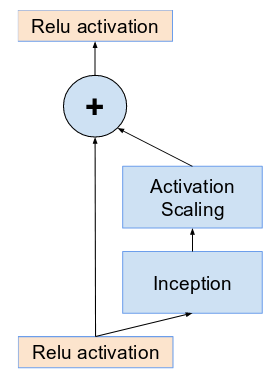
\includegraphics[height=10cm,width=9cm]{figure20.png}
    \caption{The general schema for scaling combined Inception-resnet moduels. I expect that the same idea is useful in the general resnet case, where instead of the Inception block an arbitrary subnetwork is used.  The scaling block just scales the last linear activations by a suitable constant, typically around 0.1.[~\cite{szegedy2017inception}]}
    \label{20}
\end{figure}

\subsection{Residual Inception Blocks}
\par For the residual versions of the Inception networks, Here cheaper Inception  blocks than the original Inception is used. Each Inception block is followed by filter-expansion layer (1x1 convolution  without  activation) which is used  for scaling up the dimensionality of the filter bank before the addition to match the depth of the input. This is needed to compensate for the dimensionality reduction induced by the Inception block.
\par we have tried several versions of the residual version of Inception. Only  two  of them are detailed here. The first one “Inception-ResNet-v1” roughly the computational cost of Inception-v3, while “Inception-ResNet-v2” matches the raw cost of the newly introduced Inception-v4 network. See Figure.~\ref{15} for the large scale structure of both variants. (However, the step time of Inception-v4 proved to be significantly slower in practice, probably due to the larger number of layers.)
Another  small  technical  difference  between  our  residual and non-residual Inception variants is that in the case of Inception-ResNet, we used batch-normalization only on top of the traditional layers, but not on top of the summations. It is reasonable to expect that a thorough use of batch-normalization  should be advantageous, but we wanted to keep each model replica trainable on a single GPU. It turned out that the memory footprint of layers with large activation size was consuming disproportionate amount of GPU memory. By omitting the batch-normalization on top of those layers, enable to increase the overall number
of Inception blocks substantially. we hope that with better utilization of computing resources, making this trade-off will become unnecessary.[\cite{DBLP:journals/corr/SzegedyIV16}]

\subsection{Scaling Residual blocks}
\par It is found that if the number of filters exceeded 1000, the residual variants started to exhibit instabilities and the network has just died early in the training, meaning that the last layer before the average pooling started to produce only zeros after a few tens of thousands of iterations. This could not be prevented, neither by lowering the learning rate, nor by adding an extra batch-normalization to this layer. It is found that scaling down the residuals before adding them to the previous layer activation seemed to stabilize the
training. In general we picked some scaling factors between 0.1 and 0.3 to scale the residuals before their being added to the accumulated layer activations refer Fig.~\ref{20}. A similar instability was observed in the case of very deep residual networks specifically VGG16 and VGG19, they suggested a two-phase training where the first “warm-up” phase is done with  very  low  learning  rate,  followed  by  a  second  phase with  high  learning  rate. It is found that if the number of filters is very high, then even a very low (0.00001) learning rate is not sufficient to cope with the instabilities and the training with high learning rate had a chance to destroy its effects. It is found it much more reliable to just scale the
residuals. Even  where  the  scaling  was  not  strictly  necessary,  it
never seemed to harm the final accuracy,  but it helped to stabilize the training.

\subsection{Loss Functions}
\par As mentioned earlier softmax is not suitable for obtaining discriminative features, different loss functions are experimented with inception-resnet-v2 architecture as follows,

\subsubsection{General Softmax Loss}
\par  The softmax function or normalized exponential function, is a generalization of the logistic function that squashes a k dimensional vector z of arbitrary real values to k dimensional vector $\sigma (z)$ of real values, where each entry is in range (0,1) and all entries adds up to 1 [\cite{100}], the function is given by
\begin{equation}
L_{S} = -\sum_{i=1}^{m}log (e^{W^{_{y_{i}}^{T}}x_{i}+b_{y_{i}}} / \sum_{j=1}^{n} e^{W^{_{j}^{T}}x_{i}+b_{j}})
\end{equation}

\subsubsection{Triplet Loss}
\par The embedding is represented by $ f(x) \epsilon \mathbb{R}^{d}$. It embeds an image x into a \textit{d}-dimensional Euclidean space. Additionally, I constrain this embedding to live on d-dimensional hypersphere, \textit{i.e.} $\left \|f(x)  \right \|^{_{2}} =1$ . This loss is motivated in the context of nearest neighbor classification. Here it is necessary to ensure that an image $x_{i}^{a}$ \textit{(anchor)} of specific person is closer to all other images $x_{i}^{p}$ \textit{positive} of the same person than it is to any image $x_{i}^{n}$ \textit{(negative)} of any other person [\cite{schroff2015facenet}]. Below represents in terms of equations
\begin{equation}
\left \| f(x{_{i}}^{a})-f(x{_{i}}^{p})\right \|_{2}^{2} + \alpha < \left \| f(x{_{i}}^{a})-f(x{_{i}}^{n})\right \|_{2}^{2}, \forall (f(x_{i}^{a}),f(x_{i}^{p}),f(x_{i}^{n}))\epsilon \tau 
\end{equation}

where $\alpha$ is the margin that is enforced between positive and negative pairs.
$\tau$ is the set of all possible triplets in the training set and has cardinality n. The loss that is being minimized in then 
\begin{equation}
L = \sum_{i}^{N}[\left \| f(x{_{i}}^{a})-f(x{_{i}}^{p})\right \|_{2}^{2} + \alpha - \left \| f(x{_{i}}^{a})-f(x{_{i}}^{n})\right \|_{2}^{2}]_{+}
\end{equation}

Generating all possible triplets would result in many triplets that are easily satisfied. These triplets would not contribute to the training and results in slower convergence, as they would still be passed  through the network.  It is crucial to select hard triplets, that are active and can therefore contribute to improving the model.  The following section talks about the different approaches we use for the triplet selection.
\begin{itemize}
\item Generate triplets offline every n steps, using the most recent network checkpoint and computing the argmin and argmax on a subset of the data.
\item Generate triplets online.  This can be done by selecting the hard positive/negative exemplars from within a mini-batch.
\end{itemize}

\subsubsection{Large Margin Cosine Loss}
Large margin cosine loss is similar to the softmax loss with one difference in computing the exponential value of $e^{f_{y_{i}}}$, where 
\begin{equation}
{f_{j}}=W_{j}^{T} x = \left \| W_{j} \right \|\left \| x \right \|cos\Theta _{j}
\end{equation}
where $\Theta _{j}$ is angle between $W_{j}$ and x. This formula suggests that both norm and angle of vectors contribute to posterior probability. To have the norm of W as invariable we can use L2 normalization. In testing stage the face recognition score of a testing face pair is usually calculated according to cosine similarity between the two feature vectors.  This suggests that the norm of feature vector x is not  contributing to the scoring function.  Thus, in the training stage, it assumed as $\left \| x \right \| =s$ . Consequently, the posterior probability merely relies on cosine of angle.

Considering  a  scenario  of  binary-classes  for  example, let $\theta _{i}$ denote the angle between the learned feature vector and  the  weight  vector  of  Class $C_{i}$ (i = 1,2). The Normalized softmax loss forces $\cos(\theta_{1}) > \cos(\theta_{2})$ for $C_{i}$, and similarly  for $C_{2}$ , so that features from different classes are correctly classified. To develop a large margin classifier, we further require $\cos(\theta_{1}) - m > \cos(\theta_{2})$ and $\cos(\theta_{2}) - m > \cos(\theta_{1})$ where $m \geq 0$  is a fixed parameter introduced to control the magnitude of the cosine margin. Since $\cos(\theta_{i})$ - m is lower than $\cos(\theta_{i})$, the constraint is more stringent for classification. The above analysis can be well generalized to the scenario of multi-classes.  Therefore, the altered loss reinforces the
discrimination of learned features by encouraging an extra margin in the cosine space [\cite{DBLP:journals/corr/abs-1801-09414}]. LMC can be finally defined as below

\begin{equation}
L_{lmc} = 1/N\sum_{i}^{n} -log((e^{s(\cos(\theta_{y_{i},i})-m})/
(e^{s(\cos(\theta_{y_{i},i})-m})+\sum_{j\neq y_{i}}^{n} e^{s(\cos(\theta_{j,i})})
\end{equation}


\subsubsection{Center Loss with Softmax Loss}
\begin{equation}
\centering
L_{c} = 1/2 \sum_{i=1}^{m}\left \| x{_{i}} - c_{y_{i}} \right \|_{2}^{2}
\end{equation}


\par where $c_{y_{i}} \epsilon \mathbb{R}^{d}$ ,.The above formulation effectively characterizes the intra-class variations. Ideally, the $c_{y_{i}}$ should be updated as the deep features changed. In other words, it is required to take the entire training set into account and average the features of every class in each iteration, which is inefficient even impractical. Therefore, the center loss can not be used directly. This is possibly the reason that such a center loss has never been used in CNNs until now. To address this problem, two necessary modifications are made. First, instead of updating the centers with respect to the entire training set, we perform the update based on mini-batch. In each iteration, the centers are computed by averaging the features of the corresponding classes (In this case, some of the centers may not update). Second, to avoid large perturbations caused by few mis-labelled samples, we use a scalar $\alpha$ to control the learning rate of the centers. The gradients of $L_{c}$ is computed with respect to $x{_{i}}$ and update equation of $c_{y_{i}}$ are computed as follows:
\begin{equation}
\partial L_{c} / \partial x_{i} = x_{i} - c_{y_{i}}
\end{equation}

\begin{equation}
\Delta c_{j}=\sum_{i=1}^{m} (\delta (y_{i}=j).(c_{j}-x{_i}) ) / (1+\sum_{i=1}^{m} \delta(y_{i}=j))
\end{equation}
where $\delta$ (\textit{ condition = 1}) if the condition is satisfied, and $\delta$ (\textit{condition = 0 }) if not, $\alpha$ is restricted in [0,1].Adoption of the joint supervision of softmax loss and center loss to train the CNNs for discriminative feature learning. [\cite{wen2016discriminative}] The formulation is given in below equation.

\begin{equation}
L = L_{S} + \lambda \times L_{c} 
\end{equation}

\begin{table}
  \centering
\begin{tabular}{ |p{5cm}|p{2.5cm}|p{2.5cm}|p{2.5cm}|p{2.5cm}|}
 \hline
 Networks & k & l & m & n\\
 \hline
 Inception-v4 & 192 & 224 & 256 & 384\\
 \hline
 Inception-ResNet-v1 & 192 & 192 & 256 & 384\\
 \hline
 Inception-ResNet-v2 & 256 & 256 & 384 & 384\\
 \hline
\end{tabular}
\caption{The number of filters of the Reduction-A module for the
three Inception variants presented in this thesis. The four numbers
in the colums of the paper parametrize the four convolutions of
Figure ~\ref{7}}\label{table:number_of_filters}
\end{table}

\section{Clustering Approaches}
For face embeddings obtained from trained neural network are consider as input for clustering faces, here i have analyzed five clustering approaches such as Scalable K-means [\cite{bahmani2012scalable}], GMM [\cite{cui2007easyalbum}], Rank order [\cite{ho2003clustering}], DBSCAN [\cite{schroff2015facenet}], DBSCAN + Kmeans [\cite{tian2007face}] and Chinese Whispers clustering [\cite{biemann2006chinese}]

\subsection{K-Means}
\par The k-means clustering algorithm alternates between assigning training examples to the nearest centroid and setting centroid to all the average of all assigned examples. Repeat till convergence:

For every \textit{i}. set
\begin{equation}
c^{(i)} := argmin_{j}\left \| x^{(i)} - \mu _{j} \right \|^{2}
\end{equation}
For every \textit{j}. set
\begin{equation}
\mu _{j} := (\sum_{i=1}^{m} \{ c^{(i)}=j \}x^{(i)})/(\sum_{i=1}^{m} \{ c^{(i)}=j \})
\end{equation}
Centroids are typically initialized randomly, but we instead use k-means++ [\cite{bahmani2012scalable}] to choose initial centroids

\subsection{Guassian Mixture Model(GMM)}
\par We model each training example as originating from one of \textit{k} Gaussian  distributions. Formally, specification of the joint distribution will be $p(x^{(i)},z^{(i)}) = p(x^{(i)}|z^{(i)})p(z^{(i)})$ , where $z^{(i)}$ is Multinomial $\phi$ and $x^{(i)}|z^{(i)} = j$. This latent random variable $z^{(i)}$ can take one of k values and identifies the Guassian from which $x^{(i)}$ was drawn. Parameter initialization done using k-means because random initialization performed poorly in comparison. 

The expectation-maximization algorithm is used to estimate parameters. The EM algorithm alternates between (E-step) and estimating the values of $z^{(i)}$ and (M-step) updating the parameters of model based on those estimates, formally,

Repeat till convergence

(E-Step) for each i,j, set
\begin{equation}
w_{j}^{(i)} := p(z^{(i)}=j|x^{(i)};\phi, \mu, \sum )
\end{equation}
\newline
(M-step) update the parameters:
\begin{equation}
\phi _{j} := 1/m\sum_{i=1}^{m} w_{j}^{(i)}
\end{equation}

\begin{equation}
\mu _{j} := (\sum_{i=1}^{m} w_{j}^{(i)}x^{(i)})/\sum_{i=1}^{m}w_{j}^{(i)}
\end{equation}

\begin{equation}
\sum :=( \sum_{i=1}^{m} w_{j}^{(i)}(x^{(i)}-\mu _{j})(x^{(i)}-\mu _{j})^{T}) / (\sum_{i=1}^{m} w_{j}^{(i)})
\end{equation}

\subsection{Density based clustering(DB-SCAN)}
\par The  objective  of  DBSCAN  is  to  cluster  together  high-density regions and mark low-density regions as noise. The algorithm takes two parameters: $\epsilon$,  a distance parameter, and \textit{minPts}, the minimum number of points required to
form a dense region. For each training example \textit{x}, the algorithm then (1) retrieves all \textit{n} points within an radius of \textit{x} ,(2) either adds all
\textit{n} points and their respective clusters to a new cluster if $\textit{n} \geq
\textit{minPts}$ or marks \textit{x} as noise if \textit{n} < \textit{minPts}. Note that a point marked as noise can still be assigned to a future cluster. As a modification, initialization is done as, each training example as being its own unique assignment. Then instead of labeling a point as noise, simply leave its original assignment unchanged. This ensures that every face eventually gets assigned to some unique identity.  Moreover, we iteratively test out various epsilon values for optimization and choose the epsilon value which yields the highest silhouette coefficient as a parameter.

\subsection{Rank Order Clustering}
\par Rank-Order is a form of agglomerative hierarchical clustering, meaning all training examples initially represent different clusters and are iteratively merged together. In this specific implementation, below following distance metric is used:
\begin{equation}
D(a,b) = d(a,b) + d(b,a)/ min(O_{a}(b),O_{b}(a))
\end{equation}
where,
\begin{equation}
d(a,b) = \sum_{i=1}^{min(O_{a}(b),k)} I_{b}(O_{b}(f_{a}(i)),k)
\end{equation}
$f_{a}$ is the i-th nearest face to a, $O_{b}(f_{a}(i))$ gives the rank of face $f_{a}(i)$ in face b's neighbor list, and $I_{b}(x,k)$ is 0 if face \textit{x} is in face b's top \textit{k} nearest neighbors ans 1 otherwise.

\par The  algorithm finds the k-nearest neighbors for each face \textit{a}, computes pairwise distances D(a,b) between \textit{a} and its top \textit{k} neighbors, and transitively merges all (a,b) with distances below a given threshold. It repeats
these steps until no further pairwise distances fall below this threshold.

\subsection{DBSCAN + K-means}
\par In this novel algorithm, we run DBSCAN on top of clusters already produced by
k-means.  In other words, initialization of each training example using the assignments given by k-means. When running k-means, choose an optimal $\epsilon$
to break apart too-large clusters.  For each individual cluster generated by
k-means, find optimal epsilon (based on silhouette coefficient) to run DB-SCAN on the cluster. Thus, each DBSCAN run is optimized for each individual cluster  and we achieve highly refined and distinct clusters. This provides an automated method to approximate the number of identities or clusters (i.e. k) in contrast to k-means.

\subsection{Chinese Whispers Clustering}
\par Chinese Whispers is a clustering method used in network science named after the famous whispering game. It has major implication in natural language processing. Chinese Whispers is a hard partitioning, randomized, flat clustering (no hierarchical relations between clusters) method. The random property means that running the process on the same network several times can lead to different results, while because of hard partitioning one node can only belong to one cluster at a given moment. The original algorithm is applicable to undirected, weighted and unweighted graphs. Chinese Whispers is time linear which means that it is extremely fast even if the number of nodes and links are very high in the network.[\cite{biemann2006chinese}] Here the modified version of this clustering algorithm is done. where embeddings from the neural net is gathered and every embedding is considered as node and edge is created for the nodes which are very closer each other measured using summation of least squared euclidean distance and high correlation between every embeddings in dataset.

\newpage
\chapter{Implementation}
\label{chap4}
\section{Siamese Training}
\par Siamese neural network is a class of neural network architectures that contain two or more identical subnetworks. Identical here means they have the same configuration with the same parameters and weights. Parameter updating is mirrored across both subnetworks. Siamese NNs are popular among tasks that involve finding similarity or a relationship between two comparable things. Some examples are paraphrase scoring, where the inputs are two sentences and the output is a score of how similar they are; or signature verification, where figure out whether two signatures are from the same person. Generally, in such tasks, two identical subnetworks are used to process the two inputs, and another module will take their outputs and produce the final output. Siamese architectures are good in these tasks because sharing weights across subnetworks means fewer parameters to train for, which in turn means less data required and less tendency to overfit. Each subnetwork essentially produces a representation of its input. If your inputs are of the same kind, like matching two sentences or matching two pictures, it makes sense to use similar model to process similar inputs. This way you have representation vectors with the same semantics, making them easier to compare. [\cite{bromley1993reputation}]. To visualize siamese architecture refer Figure.\ref{siamese}


\section{Deployment Overview}
To understand the complete overview of the unsupervised face recognition project refer fig ~\ref{overview}. Initial steps involves face detection and preprocessing the face images, training Deep CNN with annotated images, obtaining embeddings from trained neural network, cluster the embeddings and obtain labels and finally, retrain the model for packing embeddings tighter.

\begin{figure} [h]
    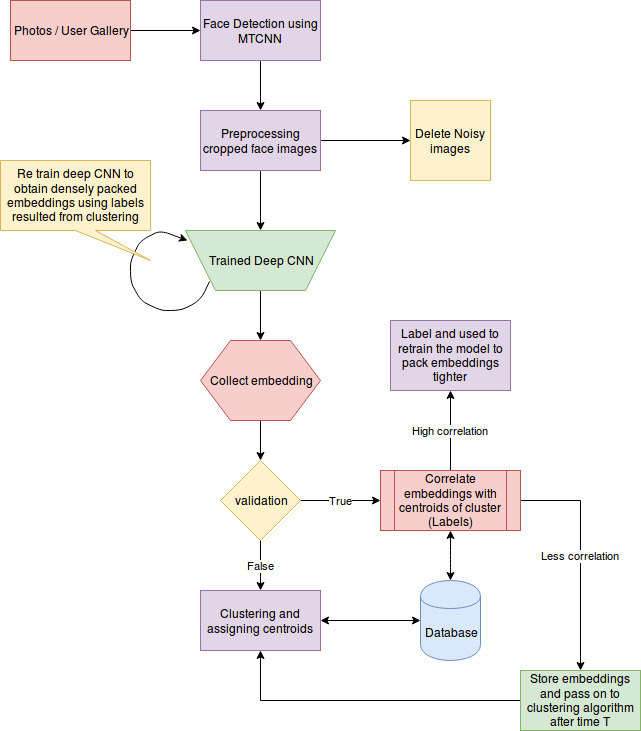
\includegraphics[height=\textheight,width=\textwidth]{overview.jpg}
    \caption{Overview of the Unsupervised face recognition}
    \label{overview}
\end{figure}

\subsection{Face Detection}
Pre-trained  multi-task  cascaded  convolutional neural  network (MTCNN)  is used   to  detect  and  align  the  faces [\cite{zhang2014jointly}]. The MTCNN framework uses a cascading  structure  with  three  stages  of  deep  convolutional networks that predict face and landmark location. Given an image, it is initially resized to different scales to build an image pyramid, which is given as the input for the three-stage cascaded framework. refer fig ~\ref{mtcnn} 
\begin{itemize}
\item In stage 1, a convolutional network called Proposal Network (P-Net) obtains the candidate windows and their bounding box regression vectors. After that, estimated bounding box regression vectors are used to calibrate the candidates.  Finally, a non-maximum suppression  (NMS)  is  used  to  merge  highly  overlapped candidates.
\item In stage 2,  all candidates are inputted into a CNN, called Refine Network (R-Net), which further rejects a  large  number  of  false  candidates,  performs  calibration with bounding box regression, and NMS candidate merge.
\item In stage 3, the network describes the face in more details and outputs five facial landmarks positions along with the aligned and cropped image. 
\end{itemize}   
\begin{figure} [h]
\centering
    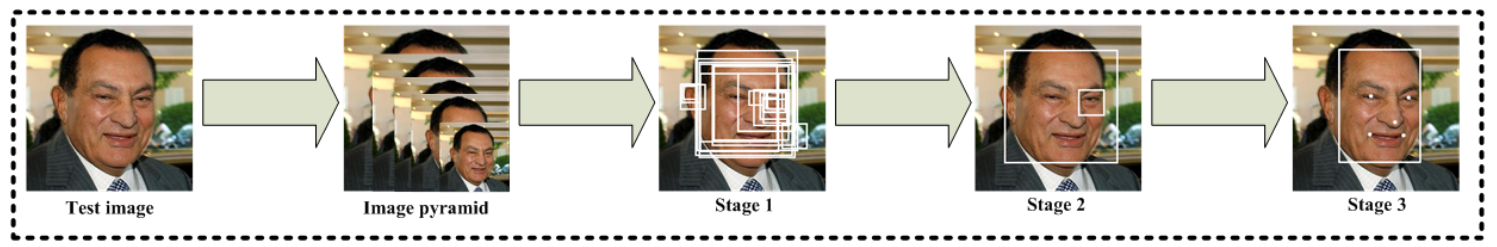
\includegraphics[height=4cm,width=15cm]{mtcnn.png}
    \caption{Overview of how MTCNN works}
    \label{mtcnn}
\end{figure}

\subsection{Supervised Face Recognition}

\subsubsection{Dataset Used}
\par Initially, face images are cropped and passed into deep CNN for training, for training initially standard datasets are used. They are CASIA-WebFace dataset consists of total of 4,53,453 images over 10,575 identities after face detection. Some performance improvement has been seen if the dataset has been filtered before training. The best performing model has been trained initially on the VGGFace2 dataset consisting of ~3.3M faces and ~9000 classes. Refer figure for Accuracy and loss on training CASIA-webface dataset ~\ref{csia_acc}, ~\ref{csia_loss} and VGG Face2 dataset refer fig ~\ref{vggface_acc}, ~\ref{vggface_loss}. Refer table ~\ref{table:acc_} for the training accuracy results.







\begin{figure}
\centering
\begin{minipage}[b]{0.4\textwidth}
   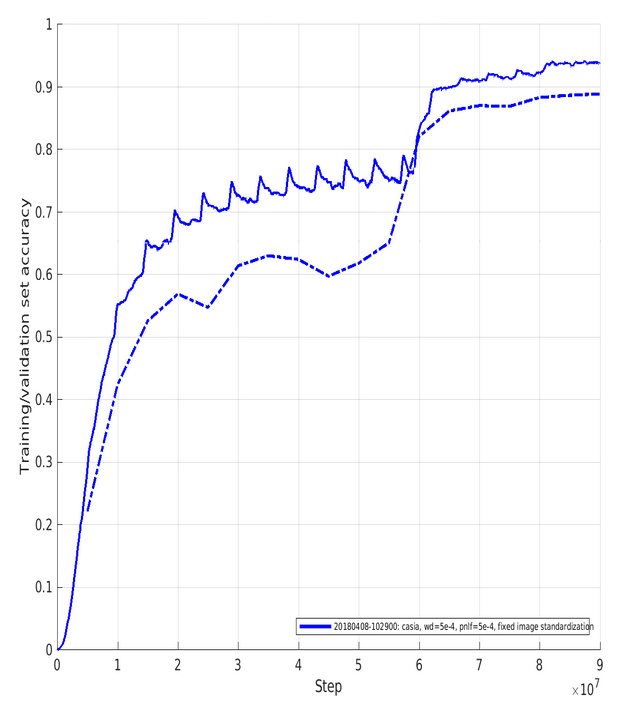
\includegraphics[width=\textwidth]{csia_acc.png}
    \caption{Training and Validation Accuracy on CASIA-webface Dataset}
    \label{csia_acc}
  \end{minipage}
  \hfill
  \begin{minipage}[b]{0.4\textwidth}
    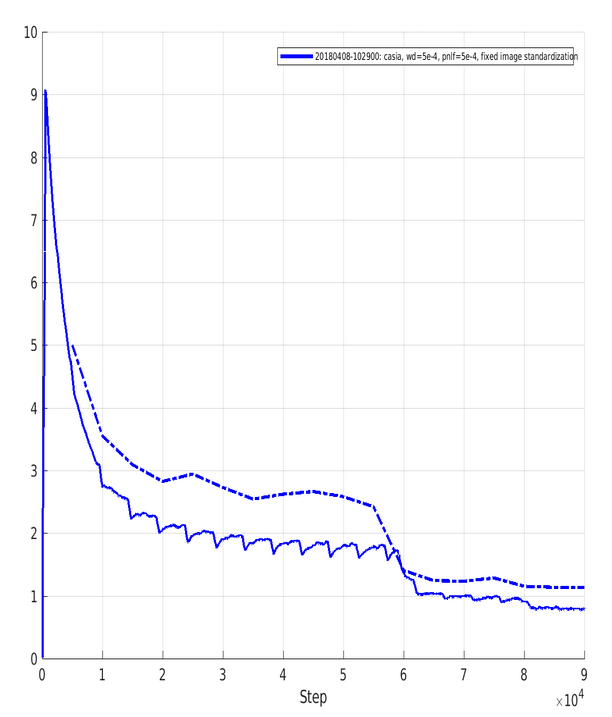
\includegraphics[width=\textwidth]{csia_loss.png}
    \caption{Training and Validation Loss on CASIA-webface Dataset}
    \label{csia_loss}
  \end{minipage}
\end{figure}

\begin{figure}
\centering
\begin{minipage}[b]{0.4\textwidth}
   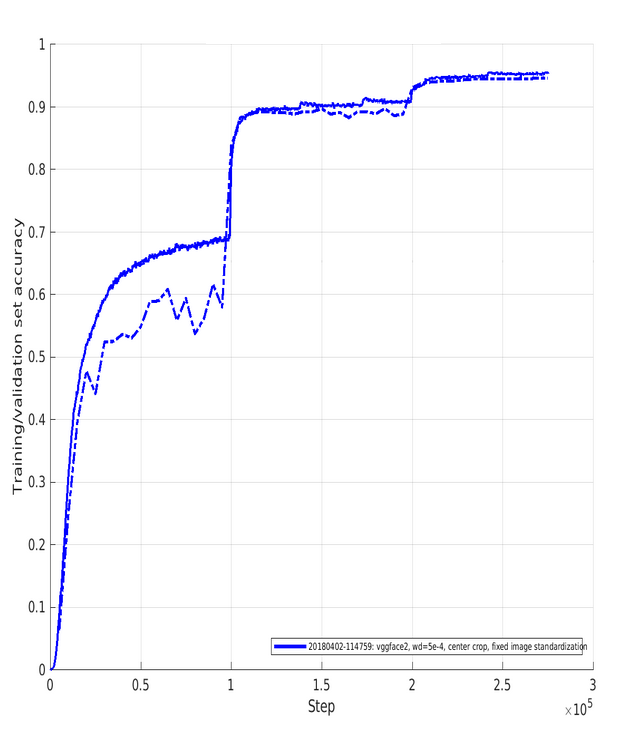
\includegraphics[width=\textwidth]{vgg_acc.png}
    \caption{Training and Validation Accuracy on VGG-face2 Dataset}
    \label{vggface_acc}
  \end{minipage}
  \hfill
  \begin{minipage}[b]{0.4\textwidth}
    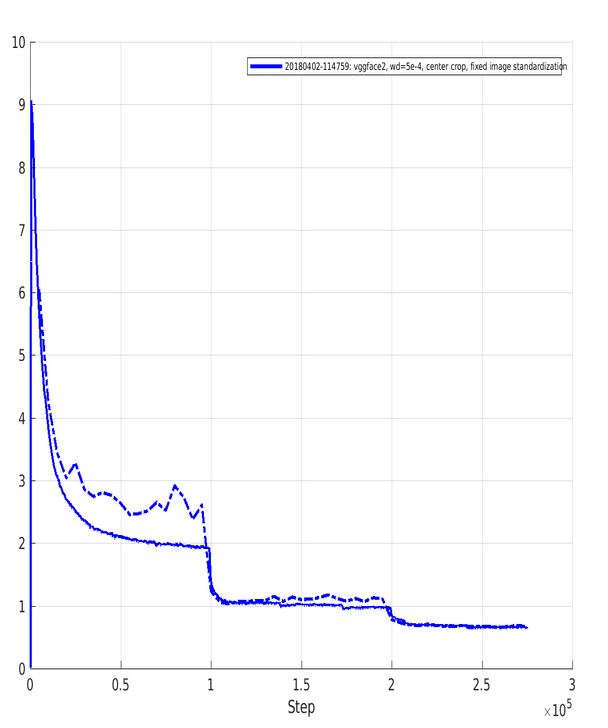
\includegraphics[width=\textwidth]{vgg_loss.png}
    \caption{Training and Validation Loss on VGG-face2 Dataset}
    \label{vggface_loss}
  \end{minipage}
\end{figure}
\newpage

\subsubsection{Algorithm for Training}
\begin{algorithm}
\caption{Algorithm for Training Deep CNN}
\begin{algorithmic} 
\STATE 1: Consider positive, anchor and negative images where positive and anchor are different instances of same person. Negative and anchor are images of different person.
\STATE 2: Choosing completely different negative image makes the convergence slower so that after N epochs, distance matrix for all images in current mini-batch is computed, and least distance with anchor and negative image is chosen. This also avoid the false convergence phenomenon of siamese network. 
\STATE 3: Training is performed by having two instance of Deep CNN model, where anchor and positive pairs, anchor and negative pairs are passed for training deep CNN. Refer Fig.\ref{triplet} results in learning process using triplet loss. Synthetic Gradients are used to train model based on only inception resnet v2 architecture. Fig.~\ref{center} shows the new extended architecture of inception resnet v2.

\STATE 4: Using pre-trained architecture of inception resnet v2, last layer (containing logits (or) vector outputting 128 embeddings) with softmax as activation function is removed and output tensor is connected according to the architecture in fig.~\ref{center}.where \textbf{C} is Convolutional Layer, \textbf{P} is Pooling Layer, \textbf{LC} is Locally Connected Layer and \textbf{FC} is Fully Connected Layer. Newly added layers weights are initialized with uniform normal distribution. This network is fine tuned with center loss. 

\STATE 5: Usage of center loss after training with triplet loss made the model to learn the facial features and makes convergence of embeddings faster. Visualization of embeddings obtained by passing images into trained neural network is performed by T-SNE. Refer fig.~\ref{embedding_vis}

\STATE 6: Once visualization of TSNE is satisfactory and can also handles high class imbalance problem. The network weights are used for clustering process.

\end{algorithmic}
\end{algorithm}

\subsection{Training steps for online training}
\par Inception Resnet v2 is one of the deep network architecture used so that training process on annotated images performed initially will have high time complexity because of the issues in convergence and over fitting of the model during online training. To avoid these issues, for the first time synthetic gradients (SC) has been implemented on CNN to compute next gradient values without actual back propagation step. Synthetic Gradients are introduces and has implications in recurrent neural networks to compute values of gates in problem of language and sequence modeling.  In a deep CNN forward pass and backward pass consume lot of time, so to prevent it, a small neural network which are densely connected are used to compute the gradient values. Refer Figure ~\ref{synthetic_grad} for the visual understanding of synthetic gradient computation [\cite{DBLP:journals/corr/JaderbergCOVGK16}]. Backward pass is also called as update lock. The objective function for the decoupled neural network is norm of squared difference between the predicted gradient and actual back-propagated gradient.

\par Tuning on real time images is also performed on custom neural network architecture with synthetic gradients, where synthetic gradients are calculated only at the larger filter sized convolutions like 17x17. This assumption is based on calculative analysis on the time complexity involved in training the neural network, refer fig.~\ref{center}. 


 
\begin{figure} [h]
\centering
    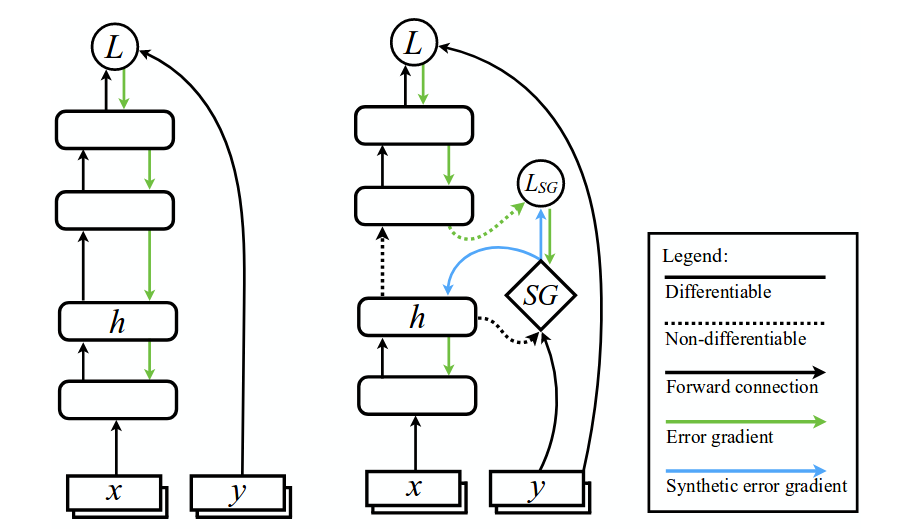
\includegraphics[height=10cm,width=14cm]{Selection_039.png}
    \caption{Back propagation without synthetic gradients and with synthetic gradients}
    \label{synthetic_grad}
\end{figure}


\subsection{Clustering}
\par Chinese whispers clustering algorithm is used to gather highly correlated face images. Refer the table ~\ref{table:cluster} for the comparative study of clustering algorithm used. Clustering algorithms executed over the training data containing 80k images and the highest-performing algorithm is executed over the testing data. Silhouette coefficient as our primary evaluation metric, where a higher silhouette coefficient is more preferred. This metric is defined for each sample \textit{x} as

\begin{equation}
s = (b-a)/max(a,b)
\end{equation}

\par where \textit{a} is the mean distance between \textit{x} and all other points
assigned to the same centroid, and \textit{b} is the mean distance between \textit{x} and all other points of the next nearest cluster. Refer figure ~\ref{tsne} for the visualization of results after clustering.

\par Thus the clustering algorithm is a graph based approach where edges are created between highly correlated embeddings obtained from the neural network, but the problem is that, the centroid of the network will not be returned as result of algorithm. In case of using mean of all the embeddings as the centroid of a particular cluster results in less accuracy if data stream into server for a time interval \textit{T} is less and also because of outliers which will affect the model on the go. To avoid that medoid for every cluster is calculated and stored in database. 

\subsubsection{Validation}
For validating input cropped faces, images are passed into deep CNN architecture and embeddings are obtained. For every instance of existing medoid in database, validation set embeddings are correlated, only correlation with more than threshold 
\textit{t} (optimal threshold found by experimentation is 0.8) will be assigned to that corresponding cluster in database, else exported embeddings are stored in separate directory until time \textit{T} to get involved in clustering algorithm again. 

\subsubsection{T-SNE}
A popular method for exploring high-dimensional data is something called t-SNE, introduced by van der Maaten and Hinton [\cite{maaten2008visualizing}] . The technique has become widespread in the field of machine learning, since it has an almost magical ability to create compelling two-dimensonal “maps” from data with hundreds or even thousands of dimensions. Tsne is used to visualize 128 dimensional vector obtained with labels as results of clustering.

\begin{table}[h]
  \centering
\begin{tabular}{ |p{4cm}|p{4cm}|p{4cm}|}
\hline
Accuracy & Training dataset & Architecture\\
\hline
0.9905 & CASIA-WebFace & Inception ResNet v2 \\
\hline
0.9965 & VGGFace2 &	Inception ResNet v2 \\
\hline
\end{tabular}
\caption{Accuracy on Public available datasets}\label{table:acc_}
\end{table}


\begin{table}[h]
  \centering
\begin{tabular}{ |p{1.5cm}|p{1.5cm}|p{3.5cm}|p{4cm}|p{2cm}|}
\hline
Accuracy & Test Accuracy & Algorithm & Tested On & \#Samples\\
\hline
0.98 & 0.96 & Chinese Whispers Clustering & Real-Time Dataset(IDrive Inc.) & 80k \\
\hline
0.84 & 0.65 & Scalable K means ++ Clustering & Real-Time Dataset & 50K \\
\hline
0.98 & 0.94 & Scalable K means ++ Clustering & CASIA and VGG Face2 & 80k \\
\hline
0.89 & NIL & GMM Clustering & VGG Face2 & 3.3M \\
\hline
0.61 & NIL & DBSCAN & VGG Face2 & 3.3M \\
\hline
\end{tabular}
\caption{Clustering Accuracy}\label{table:cluster}
\end{table}



\begin{figure} [h]
\centering
    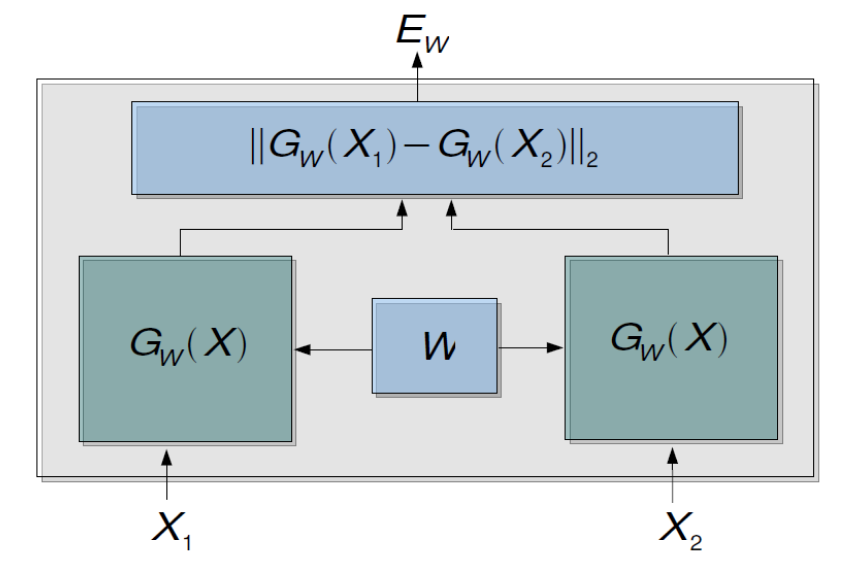
\includegraphics[height=6cm,width=10cm]{siamese.png}
    \caption{Siamese Architecture}
    \label{siamese}
\end{figure}
\begin{figure} [h]
\centering
    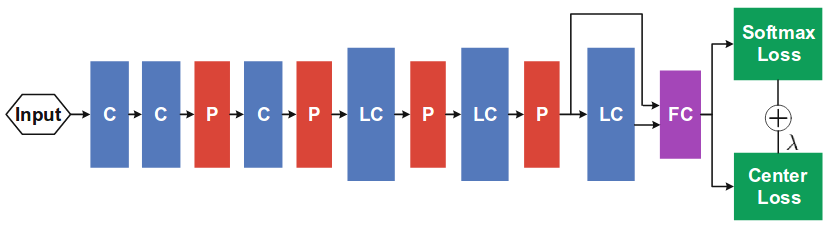
\includegraphics[height=5cm,width=15cm]{center.png}
    \caption{Training model using center loss where input is embeddings obtained from Inception-Resnet-v2, The CNN architecture using for face recognition experiments. Joint supervision is adopted. The filter sizes in both convolution and local convolution layers are 3x3 with stride 1, followed by PReLU [~\cite{DBLP:journals/corr/HeZR015}] nonlinear units. Weights in three local convolution layers are locally shared in the regions of 4x4, 2x2 and 1x1 respectively. The number of the feature maps are 128 for the convolution layers and 256 for the local convolution layers. The max-pooling grid is 2x2 and the stride is 2. The output of the 4th pooling layer and the 3th local convolution layer are concatenated as the input of the 1st fully connected layer. The output dimension of the fully connected layer is 512.}
    \label{center}
\end{figure}
\begin{figure}[h]
\centering
    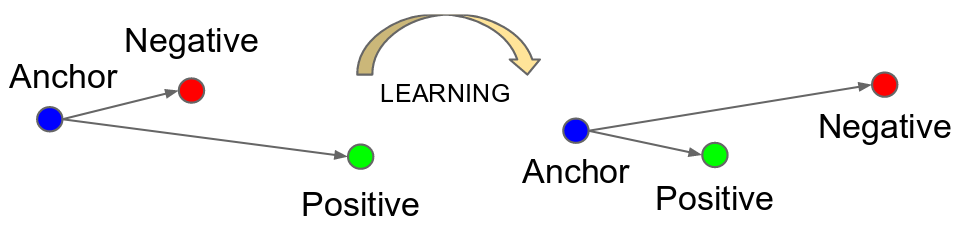
\includegraphics[height=6cm,width=13cm]{Selection_034.png}
    \caption{The Triplet Loss minimizes the distance between an anchor and a positive , both of which have the same identity, and maximizes the distance between the anchor and a negative of a different identity.}
    \label{triplet}
 
\end{figure}

\begin{figure} [h]
\centering
    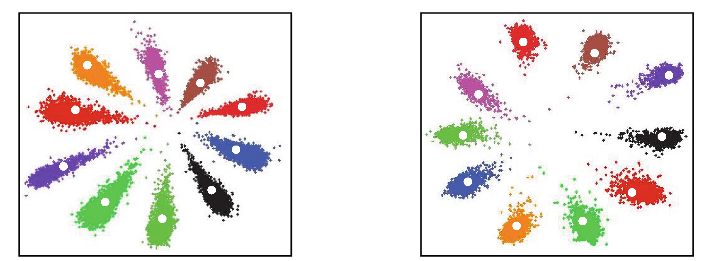
\includegraphics[height=7cm,width=10cm]{embeddings.png}
    \caption{Embeddings visualization between triplet loss and center loss using tsne}
    \label{embedding_vis}
\end{figure}

\begin{figure} [h]
\centering
    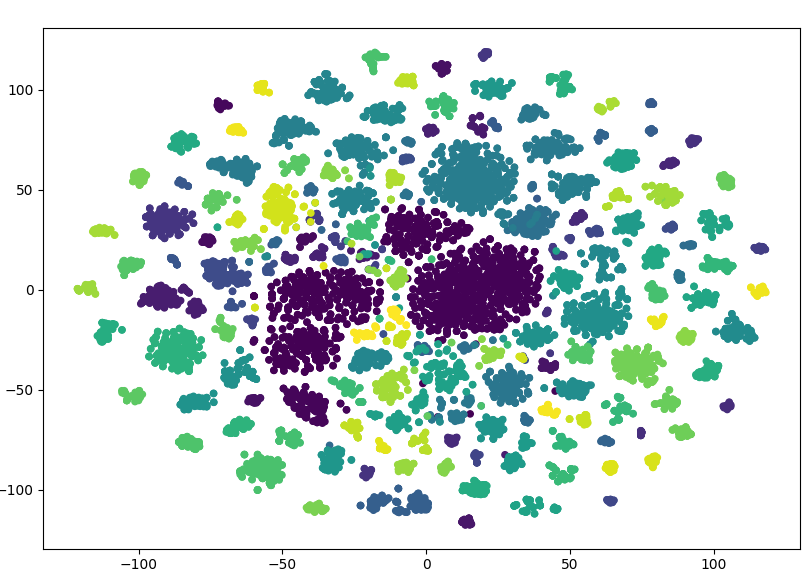
\includegraphics[height=7cm,width=10cm]{tsne_15k.png}
    \caption{T-SNE visualization for 15K images as result of chinese whispers clustering}
    \label{tsne}
\end{figure}


\newpage
\chapter{Conclusion}
\label{chap5}
\section{Conclusion and Further Research Directions}
\par The model is deployed for handling streaming data where 100k images are uploaded every hour, while deploying the model big data engines are supposed to be used for scalability. Thus by retraining the model at different instance at nodes in cloud for every \textit{T} time period with labels obtained from results of clustering, more optimal and precise face recognition results can be produced. Usage of high quality digital sources to capture images reduces the error rate in training the neural network. This research can be extended by usage of variational auto encoders or generative model to simulate and understand peoples feeling through facial expressions which adds up a factor in understanding the patterns of people behavior by Government and Business Agencies. Deep CNN model can be fine tuned to learn the behavior of primates in forests and which in turn results in understanding the ecosystem.  
	

\bibliographystyle{apalike}
\bibliography{ref.bib}


\newpage
%\pagenumbering{roman}
\pagestyle{plain}
\thispagestyle{empty}
\addcontentsline{toc}{section}{Biodata}
\chapter*{\centering BIODATA}

\begin{table}[htbp]
	\centering
	\begin{adjustbox}{center}	
		\begin{tabular}{p{4cm} p{7cm}}
			\textbf{Name} & RaviRaaja L\\
			&\\
			\textbf{Address} & 210/1 Shanthi Illam,\\
			& Vandipet street, Swaminathapuram,\\
			& Salem , TamilNadu\\
			& PIN code - 636009\\
			&\\
			
			\textbf{E-mail} & \href{mailto:mailstoraviraaja@gmail.com}{mailstoraviraja@gmail.com}\\
			&\\
			
			\textbf{Mobile} & 9626161704\\
			&\\
			
			\textbf{Qualification} & B.Tech. in Information Technology\\
			& (Anna University, Chennai)\\
			&\\ 
            & M.Tech. in Computer Science and Engineering - Information Security\\
			& (NITK Surathkal)\\
		\end{tabular}
	\end{adjustbox}
\end{table}




\end{document}




